\chapter{Color representation}

This part extracts infromation from the course book Digital Image Processing, Gonzales \cite{diProcessing} unless other sources stated.

\section{Primary Colors}

The use of images is a great way of providing information visually. An image is represented by a rectangular grid where each cell, or hereafter pixel, emits light of a certain wavelength. When the color of each pixel is determined and is ready to be displayed, there is a problem of how to convey the color information from the source to the recipients eyes. On way would be to many different light sources for each pixel, where each source is responsible for a small region of wavelengths. This is problematic due to our wide range of visible colors and in order to reduce the number of light sources we need, these wavelength regions must be chosen with care. This problem is slightly simplified by the fact that our eyes consists of three different sensors that react to different wavelengths, and these are roughly equal to blue, green and red colors and their absorption can be seen in Fig.~\ref{fig:colorAbsorption}.

\begin{figure}[h]
    \centering
    \resizebox{0.49\textwidth}{!}{
        % This file was created by matlab2tikz.
%
%The latest updates can be retrieved from
%  http://www.mathworks.com/matlabcentral/fileexchange/22022-matlab2tikz-matlab2tikz
%where you can also make suggestions and rate matlab2tikz.
%
\begin{tikzpicture}

\begin{axis}[%
width=4.521in,
height=3.53in,
at={(0.758in,0.517in)},
scale only axis,
xmin=390,
xmax=850,
xlabel={Wavelength, $\lambda\;[nm]$},
ymin=0,
ymax=1,
ytick={\empty},
ylabel={Intensity, $I$},
axis background/.style={fill=white},
title style={font=\bfseries},
title={Intensity ranges for RGB color channels},
legend style={at={(0.97,0.03)},anchor=south east,legend cell align=left,align=left,draw=white!15!black}
]
\addplot [color=blue,dashdotted]
  table[row sep=crcr]{%
390	0\\
391	4.07641293463662e-07\\
392	6.37175299352561e-06\\
393	3.15068671549313e-05\\
394	9.72435132307244e-05\\
395	0.000231803023544704\\
396	0.000469222789545911\\
397	0.000848431011784255\\
398	0.00141236998654636\\
399	0.00220716697209077\\
400	0.00328135167742148\\
401	0.00468511941653912\\
402	0.00646963897110858\\
403	0.0086864042044825\\
404	0.0113866284700194\\
405	0.0146206808566358\\
406	0.0184375633145313\\
407	0.0228844277040258\\
408	0.0280061318104477\\
409	0.0338448333680121\\
410	0.0404396211356295\\
411	0.047826182067582\\
412	0.0560365036220067\\
413	0.0650986102501267\\
414	0.0750363331091675\\
415	0.0858691120418978\\
416	0.0976118288657348\\
417	0.110274671014352\\
418	0.12386302457473\\
419	0.138377395762587\\
420	0.153813359879131\\
421	0.170161536792071\\
422	0.187407591983826\\
423	0.205532262209874\\
424	0.224511404810172\\
425	0.244316069716601\\
426	0.264912593199353\\
427	0.286262712395227\\
428	0.308323699660747\\
429	0.331048515793055\\
430	0.354385981161518\\
431	0.37828096379298\\
432	0.40267458345361\\
433	0.427504430770273\\
434	0.452704800434371\\
435	0.478206937531092\\
436	0.503939296037\\
437	0.529827808528918\\
438	0.555796166147025\\
439	0.581766107855124\\
440	0.607657718041012\\
441	0.633389731499878\\
442	0.658879844843709\\
443	0.684045033379583\\
444	0.708801872499845\\
445	0.733066862627069\\
446	0.756756756756757\\
447	0.779788889640723\\
448	0.802081507654077\\
449	0.823554098388778\\
450	0.84412771901667\\
451	0.863725322464952\\
452	0.882272080447028\\
453	0.899695702391651\\
454	0.915926749313333\\
455	0.930898941666932\\
456	0.944549460229374\\
457	0.956819239051439\\
458	0.967653249522547\\
459	0.977000774591503\\
460	0.984815672186114\\
461	0.991056626874631\\
462	0.995687388811958\\
463	0.998676999013557\\
464	1\\
465	0.999636630855092\\
466	0.997573005740522\\
467	0.993801274909959\\
468	0.988319767265562\\
469	0.98113311349981\\
470	0.972252348865616\\
471	0.961694994617654\\
472	0.949485117167833\\
473	0.935653363997875\\
474	0.920236975371912\\
475	0.903279770892061\\
476	0.884832109939905\\
477	0.864950825046829\\
478	0.843699127236133\\
479	0.821146482379881\\
480	0.797368457613413\\
481	0.77244653685046\\
482	0.746467904441805\\
483	0.719525196020432\\
484	0.691716215576085\\
485	0.6631436178022\\
486	0.633914554758133\\
487	0.60414028588963\\
488	0.573935750450468\\
489	0.543419101368225\\
490	0.512711199597101\\
491	0.481935068000731\\
492	0.451215303807943\\
493	0.420677448684378\\
494	0.390447315462937\\
495	0.360650270575969\\
496	0.331410471232154\\
497	0.302850056381022\\
498	0.275088290508031\\
499	0.248240659303162\\
500	0.22241791624596\\
501	0.197725079149963\\
502	0.174260375709451\\
503	0.152114137091465\\
504	0.131367638616035\\
505	0.11209188656754\\
506	0.0943463501801598\\
507	0.0781776378403416\\
508	0.0636181165492335\\
509	0.0506844736880133\\
510	0.0393762201290571\\
511	0.0296741337358864\\
512	0.0215386422948316\\
513	0.0149081449213515\\
514	0.00969727098394851\\
515	0.00579507558861736\\
516	0.00306317066676766\\
517	0.00133379070955866\\
518	0.000407792191585641\\
519	5.25857268568126e-05\\
520	0\\
};
\addlegendentry{Blue channel};

\addplot [color=green,solid]
  table[row sep=crcr]{%
480	0\\
481	0.00093223626623717\\
482	0.00367135604495638\\
483	0.00813198417422354\\
484	0.0142300899828436\\
485	0.0218829872903608\\
486	0.0310093344070584\\
487	0.0415291341339586\\
488	0.0533637337628231\\
489	0.0664358250761532\\
490	0.0806694443471871\\
491	0.0959899723399044\\
492	0.112324134309023\\
493	0.1296\\
494	0.147746983649032\\
495	0.166695843983054\\
496	0.18637868421974\\
497	0.206728952067505\\
498	0.2276814397255\\
499	0.249172283883617\\
500	0.271138965722488\\
501	0.293520310913483\\
502	0.31625648961871\\
503	0.339289016491019\\
504	0.362560750673997\\
505	0.386015895801968\\
506	0.409600000000001\\
507	0.433259955883898\\
508	0.456944000560205\\
509	0.480601715626204\\
510	0.504184027169917\\
511	0.527643205770106\\
512	0.550932866496271\\
513	0.574007968908652\\
514	0.596824817058226\\
515	0.619341059486712\\
516	0.641515689226567\\
517	0.663309043800987\\
518	0.684682805223906\\
519	0.7056\\
520	0.72602499912468\\
521	0.7459235180841\\
522	0.765262616855152\\
523	0.784010699905465\\
524	0.80213751619341\\
525	0.819614159168096\\
526	0.83641306676937\\
527	0.85250802142782\\
528	0.867874150064773\\
529	0.882487924092294\\
530	0.896327159413187\\
531	0.909371016420994\\
532	0.921600000000001\\
533	0.932995959525227\\
534	0.943542088862435\\
535	0.953222926368125\\
536	0.962024354889535\\
537	0.969933601764644\\
538	0.97693923882217\\
539	0.983031182381569\\
540	0.988200693253038\\
541	0.992440376737509\\
542	0.995744182626659\\
543	0.998107405202899\\
544	0.999526683239382\\
545	1\\
546	0.999526683239382\\
547	0.998107405202899\\
548	0.995744182626659\\
549	0.992440376737509\\
550	0.988200693253038\\
551	0.983031182381569\\
552	0.97693923882217\\
553	0.969933601764644\\
554	0.962024354889535\\
555	0.953222926368125\\
556	0.943542088862435\\
557	0.932995959525227\\
558	0.921600000000001\\
559	0.909371016420994\\
560	0.896327159413185\\
561	0.882487924092293\\
562	0.867874150064773\\
563	0.85250802142782\\
564	0.83641306676937\\
565	0.819614159168096\\
566	0.80213751619341\\
567	0.784010699905465\\
568	0.765262616855152\\
569	0.7459235180841\\
570	0.72602499912468\\
571	0.7056\\
572	0.684682805223906\\
573	0.663309043800987\\
574	0.641515689226567\\
575	0.619341059486712\\
576	0.596824817058226\\
577	0.574007968908652\\
578	0.550932866496271\\
579	0.527643205770106\\
580	0.504184027169917\\
581	0.480601715626204\\
582	0.456944000560205\\
583	0.433259955883898\\
584	0.409600000000001\\
585	0.386015895801968\\
586	0.362560750673997\\
587	0.33928901649102\\
588	0.316256489618712\\
589	0.293520310913484\\
590	0.27113896572249\\
591	0.249172283883619\\
592	0.227681439725501\\
593	0.206728952067503\\
594	0.186378684219739\\
595	0.166695843983053\\
596	0.147746983649031\\
597	0.129599999999999\\
598	0.112324134309022\\
599	0.0959899723399034\\
600	0.0806694443471862\\
601	0.0664358250761524\\
602	0.0533637337628231\\
603	0.0415291341339586\\
604	0.0310093344070584\\
605	0.0218829872903608\\
606	0.0142300899828436\\
607	0.00813198417422354\\
608	0.00367135604495638\\
609	0.00093223626623717\\
610	0\\
};
\addlegendentry{Green channel};

\addplot [color=red,dashed]
  table[row sep=crcr]{%
590	0\\
591	8.63078345051999e-05\\
592	0.000665471157595194\\
593	0.0021639294788854\\
594	0.00494023562827531\\
595	0.00928990852546671\\
596	0.0154501014943457\\
597	0.0236040892038243\\
598	0.0338855763167238\\
599	0.0463828309282881\\
600	0.0611426458759317\\
601	0.0781741310017884\\
602	0.097452339449671\\
603	0.11892173107801\\
604	0.142499476070392\\
605	0.168078601825257\\
606	0.195530986206339\\
607	0.224710200235498\\
608	0.255454203309448\\
609	0.287587894022025\\
610	0.32092551967359\\
611	0.35527294754912\\
612	0.390429801046583\\
613	0.426191463737235\\
614	0.462350954439359\\
615	0.498700676387081\\
616	0.535034043575825\\
617	0.57114698736604\\
618	0.606839346426733\\
619	0.641916143100416\\
620	0.676188749271104\\
621	0.709475944816867\\
622	0.74160487172859\\
623	0.772411886976525\\
624	0.801743317206189\\
625	0.829456118345222\\
626	0.855418443202811\\
627	0.879510120143227\\
628	0.901623045915099\\
629	0.921661495717995\\
630	0.939542353587918\\
631	0.955195266183289\\
632	0.968562723053004\\
633	0.979600066468183\\
634	0.988275433899161\\
635	0.994569636219339\\
636	0.998475974717474\\
637	1\\
638	0.99915921586496\\
639	0.995982731229157\\
640	0.990510863190095\\
641	0.982794694304307\\
642	0.972895587163663\\
643	0.960884659351242\\
644	0.946842221858355\\
645	0.930857184044319\\
646	0.913026428220557\\
647	0.893454156940628\\
648	0.872251216077767\\
649	0.84953439677152\\
650	0.825425719325078\\
651	0.800051702134897\\
652	0.773542618734163\\
653	0.746031746031745\\
654	0.717654606828184\\
655	0.688548209690312\\
656	0.658850289266108\\
657	0.62869855012137\\
658	0.598229917179797\\
659	0.567579795848042\\
660	0.536881344907381\\
661	0.506264765253546\\
662	0.475856607566303\\
663	0.445779101990402\\
664	0.416149512909475\\
665	0.387079521894437\\
666	0.35867464190803\\
667	0.331033665847082\\
668	0.304248152504037\\
669	0.278401953029404\\
670	0.253570780976664\\
671	0.22982182901126\\
672	0.207213435365226\\
673	0.185794803119073\\
674	0.165605775392517\\
675	0.146676669525612\\
676	0.129028173331914\\
677	0.112671306505246\\
678	0.0976074502616458\\
679	0.083828448298106\\
680	0.0713167821496866\\
681	0.0600458240265766\\
682	0.0499801702127182\\
683	0.0410760581075641\\
684	0.0332818699925684\\
685	0.026538726603988\\
686	0.0207811735935988\\
687	0.0159379639589085\\
688	0.0119329395244495\\
689	0.00868601455575423\\
690	0.00611426458759316\\
691	0.00413312354806529\\
692	0.00265769226013509\\
693	0.00160416140220165\\
694	0.000891352009289179\\
695	0.0004423765964508\\
696	0.000186423985972652\\
697	6.06709199687497e-05\\
698	1.23235399554668e-05\\
699	7.91814995460526e-07\\
700	0\\
};
\addlegendentry{Red channel};

\end{axis}
\end{tikzpicture}%
    }
    \caption{\label{fig:colorAbsorption}When incoming photons with different wavelengths $\lambda$ hits each receptor, they get excited depending on their ranges. The figure shows, not accurate ranges nor intensities, but illustrates a schematically the different ranges for the different colors. }
\end{figure}

These three colors, red, green, and blue are therefore called the \textit{primary colors} and will be the basis for image representations. There are two different ways of using these colors to provide the targeted color, in a additive or a subtractive manner. When adding the primaries we start with a completely black canvas and increase the intensity for each of the colors until we reach a white color. For the subtractive nature we start with a white canvas and determine how much of each color we want to subtract until a black color is reached. The difference between these can be thought of as absorption and emittance, and the distinction can be seen in Fig.~\ref{fig:color_arithmetic}.

\begin{figure}[H]
    \centering
    \captionsetup[subfigure]{justification=centering}
    \begin{subfigure}[b]{0.49\textwidth}
        \centering
        \tikzstyle{blueCircle} = [draw=none, circle, rounded corners=1em,bottom color=blue!5, top color=blue!40,
    minimum height=\R*\overlap cm,shade, minimum width=\R*\overlap cm,node distance=4 cm]
    \tikzstyle{greenCircle} = [draw=none, circle, rounded corners=1em,bottom color=green!5, top color=green!40,
    minimum height=\R*\overlap cm,shade, minimum width=\R*\overlap cm,node distance=4 cm]
    \tikzstyle{redCircle} = [draw=none, circle, rounded corners=1em,bottom color=red!5, top color=red!40,
    minimum height=\R*\overlap cm,shade, minimum width=\R*\overlap cm,node distance=4 cm]
        \tikzstyle{cyanCircle} = [draw=none, circle, rounded corners=1em,bottom color=cyan!5, top color=cyan!100,
    minimum height=\R*\overlap cm,shade, minimum width=\R*\overlap cm,node distance=4 cm]
    \tikzstyle{yellowCircle} = [draw=none, circle, rounded corners=1em,bottom color=yellow!5, top color=yellow!100,
    minimum height=\R*\overlap cm,shade, minimum width=\R*\overlap cm,node distance=4 cm]
    
    \tikzstyle{magentaCircle} = [draw=none, circle, rounded corners=1em,bottom color=magenta!5, top color=magenta!100,
    minimum height=\R*\overlap cm,shade, minimum width=\R*\overlap cm,node distance=4 cm]
    
        \tikzstyle{whiteCircle} = [draw=none, circle, rounded corners=1em,bottom color=white!5, top color=white!100,
    minimum height=\R*\overlap cm,shade, minimum width=\R*\overlap cm,node distance=4 cm]
    
\tikzstyle{shadowCircle} = [draw=black, circle, rounded corners=1em,
	blur shadow={shadow blur steps=10,shadow blur extra rounding=1.3pt},
    minimum height=\R*\overlap*1.01 cm,shade, minimum width=\R*\overlap*1.01 cm,node distance=4 cm]
\begin{tikzpicture}[auto, on grid, node distance=4cm,>=stealth]
	every node./style={rounded corners}

\newcommand\R{1}
\newcommand\overlap{3.5}

\coordinate (C) at (-\R,-{\R/sqrt(3)});
\coordinate (c1) at (0,0)+(C);
\coordinate (c2) at (\R*2,0)+(C);
\coordinate (c3) at (\R,{\R*sqrt(3)})+(C);

\node[shadowCircle] (circle1) at (c1) {};
\node[shadowCircle] (circle2) at (c2) {};
\node[shadowCircle] (circle3) at (c3) {};

\node[blueCircle] (circle1) at (c1) {};
\node[greenCircle] (circle2) at (c2) {};
\node[redCircle] (circle3) at (c3) {};

%\node[ColorCircle] (c1);
%	\node [block] (image) {$f(x,y)$};

\begin{scope}
  \clip (c1) circle (\R/2*\overlap cm);
  \node[cyanCircle] (intersect1) at (c2) {};
\end{scope}

\begin{scope}
  \clip (c2) circle (\R/2*\overlap cm);
  \node[yellowCircle] (intersect2) at (c3) {};
\end{scope}

\begin{scope}
  \clip (c1) circle (\R/2*\overlap cm);
  \node[magentaCircle] (intersect3) at (c3) {};
\end{scope}

\begin{scope}
  \clip (c1) circle (\R/2*\overlap cm);
  \clip (c2) circle (\R/2*\overlap cm);
  \node[whiteCircle] (intersect3) at (c3) {};
\end{scope}

\end{tikzpicture}


		\caption{}
		\label{fig:color_additive}
    \end{subfigure}
    \begin{subfigure}[b]{0.49\textwidth}
        \centering
        \tikzstyle{blueCircle} = [draw=none, circle, rounded corners=1em,bottom color=blue!5, top color=blue!80,
    minimum height=\R*\overlap cm,shade, minimum width=\R*\overlap cm,node distance=4 cm]
    \tikzstyle{greenCircle} = [draw=none, circle, rounded corners=1em,bottom color=green!5, top color=green!80,
    minimum height=\R*\overlap cm,shade, minimum width=\R*\overlap cm,node distance=4 cm]
    \tikzstyle{redCircle} = [draw=none, circle, rounded corners=1em,bottom color=red!5, top color=red!80,
    minimum height=\R*\overlap cm,shade, minimum width=\R*\overlap cm,node distance=4 cm]
        \tikzstyle{cyanCircle} = [draw=none, circle, rounded corners=1em,bottom color=cyan!5, top color=cyan!40,
    minimum height=\R*\overlap cm,shade, minimum width=\R*\overlap cm,node distance=4 cm]
    \tikzstyle{yellowCircle} = [draw=none, circle, rounded corners=1em,bottom color=yellow!5, top color=yellow!40,
    minimum height=\R*\overlap cm,shade, minimum width=\R*\overlap cm,node distance=4 cm]
    
    \tikzstyle{magentaCircle} = [draw=none, circle, rounded corners=1em,bottom color=magenta!5, top color=magenta!40,
    minimum height=\R*\overlap cm,shade, minimum width=\R*\overlap cm,node distance=4 cm]
    
        \tikzstyle{blackCircle} = [draw=none, circle, rounded corners=1em,bottom color=black!55, top color=black!100,
    minimum height=\R*\overlap cm,shade, minimum width=\R*\overlap cm,node distance=4 cm]
    
\tikzstyle{shadowCircle} = [draw=black, circle, rounded corners=1em,
	blur shadow={shadow blur steps=10,shadow blur extra rounding=1.3pt},
    minimum height=\R*\overlap*1.01 cm,shade, minimum width=\R*\overlap*1.01 cm,node distance=4 cm]
\begin{tikzpicture}[auto, on grid, node distance=4cm,>=stealth]
	every node./style={rounded corners}

\newcommand\R{1}
\newcommand\overlap{3.5}

\coordinate (C) at (-\R,-{\R/sqrt(3)});
\coordinate (c1) at (0,0)+(C);
\coordinate (c2) at (\R*2,0)+(C);
\coordinate (c3) at (\R,{\R*sqrt(3)})+(C);

\node[shadowCircle] (circle1) at (c1) {};
\node[shadowCircle] (circle2) at (c2) {};
\node[shadowCircle] (circle3) at (c3) {};

\node[cyanCircle] (circle1) at (c1) {};
\node[yellowCircle] (circle2) at (c2) {};
\node[magentaCircle] (circle3) at (c3) {};

%\node[ColorCircle] (c1);
%	\node [block] (image) {$f(x,y)$};

\begin{scope}
  \clip (c1) circle (\R/2*\overlap cm);
  \node[blueCircle] (intersect1) at (c3) {};
\end{scope}

\begin{scope}
  \clip (c2) circle (\R/2*\overlap cm);
  \node[greenCircle] (intersect2) at (c1) {};
\end{scope}

\begin{scope}
  \clip (c3) circle (\R/2*\overlap cm);
  \node[redCircle] (intersect3) at (c2) {};
\end{scope}

\begin{scope}
  \clip (c1) circle (\R/2*\overlap cm);
  \clip (c2) circle (\R/2*\overlap cm);
  \node[blackCircle] (intersect3) at (c3) {};
\end{scope}

\end{tikzpicture}


		\caption{}
		\label{fig:color_subtractive}
    \end{subfigure}
    \caption{Combining colors can either be done additively  (\textit{(a)}: The normal \textbf{RGB} color space combines \textcolor{red}{red} and \textcolor{blue}{blue} to \textcolor{magenta}{magenta},\textcolor{blue}{blue} and \textcolor{green}{green} to \textcolor{cyan}{cyan}, \textcolor{green}{green} and \textcolor{red}{red} to \textcolor{yellow}{yellow}, and all three to white) or subtractively (\textit{(b)}: the \textbf{CMY} color space combines colors subtractively by removing the selected colors from a pure white color).}
    \label{fig:color_arithmetic}
\end{figure}

\section{Color Spaces}

\subsection{\textbf{RGB} and \textbf{CMY}}

In the introduction of this appendix we talked about the primary colors and how they are used to represent a wide range of colors. This representation of colors is the \textbf{RGB} (red, green, blue) color space for the additive colors, and \textbf{CMY} (cyan, magenta, yellow) for the subtractive. Many other color spaces exists and are used in different situations. Ultimately they represents the same color, only through other variables than red, green, and blue. Often the change of color spaces is done by changing the basis for the color representations. E.g. transforming from \textbf{RGB} to \textbf{CMY} color space is done by the linear transformation,

\begin{equation}
\left(\begin{array}{c}
c \\ m \\ y
\end{array}\right) = 1- \left(\begin{array}{c}
r \\ g \\ b
\end{array}\right),
\end{equation}

which makes it clear why the other is called subtractive when the first is additive. Although we can change the color space in which we represent an image, the fact that our screens use red, green, and blue colors to mix colors is still present. So to view a new color space we simply use these light sources and pretend that our new values still lies in a \textbf{RGB} color space. The result of this representation can be seen in Fig.~\ref{fig:rgbTocmy}.

\begin{figure}[H]
    \centering
    \captionsetup[subfigure]{justification=centering}
    \begin{subfigure}[b]{0.49\textwidth}
        \centering
        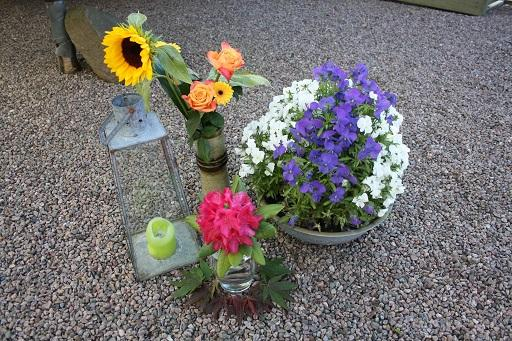
\includegraphics[width=\textwidth]{./figure/appendix/color_rep/images/imgRGB.jpg}
		\caption{}
		\label{fig:imgRGB}
    \end{subfigure}
    \begin{subfigure}[b]{0.49\textwidth}
        \centering
        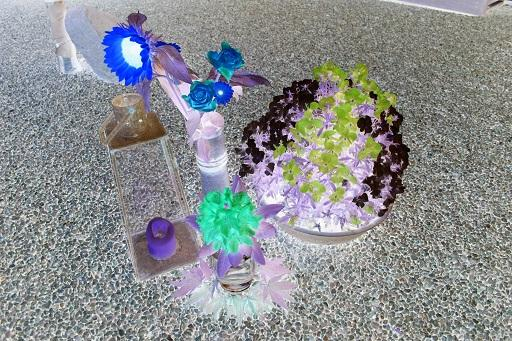
\includegraphics[width=\textwidth]{./figure/appendix/color_rep/images/imgCMY.jpg}
		\caption{}
		\label{fig:imgCMY}
    \end{subfigure}
    \caption{Presenting images using other color spaces than the ordinary \textbf{RGB} color space can yield interesting result. \textit{(a)}: Image show in the ordinary \textbf{RGB} color space. \textit{(b)}: The same image as in \textit{(a)} but show in \textbf{RGB} representation using \textbf{CMY} color values.}
    \label{fig:rgbTocmy}
\end{figure}

Sometimes the information that is interesting in the image in not needed to be expressed using three color channels and a color conversion might only produce a single index for each pixel. These will be called color indices, and basically any color space is build by three different color indices, due to the three different kinds of receptors. The difference between three random color indices and a color space is that the color space spans the entire "color room", meaning that a color space can represent any color and conversion between spaces exists, which is not always true for color indices. Several color spaces/indices will be presented as well as some reason why using them.

\subsection{HSI}

In many computer vision applications there is a need to separate segments of images based on the color of these. This could be tedious if done using the \textbf{RGB} color space. E.g. suppose you would want to select a yellowish color, but you care not for an exact color and allow some deviation. A color value is chosen as base, and small deviations in the red color channel will yield about the same color, but also small deviations in the green and blue channels will produce almost the same result. So to select the appropriate range of colors that are representative is dependent on three different deviations, and the target lies in a three dimensional shape. So a color space in which the information of the color is embedded in one of the channels could prove useful.  We can imagine that all available colors are represented on a disk where the colors changes on the viewing angle from the origin, and the prevalence of this color increases with distance. So to choose a specific color we would simply choose an angle from the origin which points at the targeted color. Then we would go in that direction until the amount of color is reached and then we increase/decrease the intensity of the selected color. This is a new color space which we call \textbf{HSI}, \textbf{H}ue, \textbf{S}aturation, and \textbf{I}ntensity. The color coordinates for this color space is here represented by an angle, a radius and a height compared to three distances for the \textbf{RGB} color space, the differences is show in Fig. ~\ref{fig:color_coordinate}

\begin{figure}[H]
    \centering
    \captionsetup[subfigure]{justification=centering}
    \begin{subfigure}[b]{0.49\textwidth}
        \centering
        \definecolor{colorRed}{rgb}{1.0,0.0,0.0}%
\definecolor{colorGreen}{rgb}{0.0,1.0,0.0}%
\definecolor{colorRedGreen}{rgb}{1.0,1.0,0.0}%
\definecolor{colorBlue}{rgb}{0.0,0.0,1.0}%
\definecolor{colorRedBlue}{rgb}{1.0,0.0,1.0}%
\definecolor{colorGreenBlue}{rgb}{0.0,1.0,1.0}%
\definecolor{colorRedGreenBlue}{rgb}{1.0,1.0,1.0}%
\begin{tikzpicture}[]
    \begin{axis}[
        set layers,
        axis equal,
        view={125}{30},
        axis lines=none,
        clip=false]
        \draw[draw=none,shade,fill =white!100,opacity=0,blur shadow={shadow blur steps=10,shadow blur extra rounding=1.3pt}] (0,0,0) -- (1.0,0,0) -- ( 1.0,1.0,0) -- (0,1.0,0);
        \addplot3[patch,
            shader=interp,
            mesh/color input=explicit]
        coordinates {
            % Red green face
            (0,0,0) [color=black!40]
            (1,0,0) [color=colorRed!40]
            (0,1,0) [color=colorGreen!40]
            (1,0,0) [color=colorRed!40]
            (0,1,0) [color=colorGreen!40]
            (1,1,0) [color=colorRedGreen!40]
            % Red blue face
            (0,0,0) [color=black!40]
            (1,0,0) [color=colorRed!40]
            (0,0,1) [color=colorBlue!40]
            (1,0,0) [color=colorRed!40]
            (0,0,1) [color=colorBlue!40]
            (1,0,1) [color=colorRedBlue!40]
            % Green blue face
            (0,0,0) [color=black!40]
            (0,1,0) [color=colorGreen!40]
            (0,0,1) [color=colorBlue!40]
            (0,1,0) [color=colorGreen!40]
            (0,0,1) [color=colorBlue!40]
            (0,1,1) [color=colorGreenBlue!40]
            % Green blue face full red
            (1,0,0) [color=colorRed!40]
            (1,1,0) [color=colorRedGreen!40]
            (1,0,1) [color=colorRedBlue!40]
            (1,1,0) [color=colorRedGreen!40]
            (1,0,1) [color=colorRedBlue!40]
            (1,1,1) [color=colorRedGreenBlue!40]
            % Red blue face full Green
            (0,1,0) [color=colorGreen!40]
            (1,1,0) [color=colorRedGreen!40]
            (0,1,1) [color=colorGreenBlue!40]
            (1,1,0) [color=colorRedGreen!40]
            (0,1,1) [color=colorGreenBlue!40]
            (1,1,1) [color=colorRedGreenBlue!40]
            % Red green face full blue
            (0,0,1) [color=colorBlue!40]
            (1,0,1) [color=colorRedBlue!40]
            (0,1,1) [color=colorGreenBlue!40]
            (1,0,1) [color=colorRedBlue!40]
            (0,1,1) [color=colorGreenBlue!40]
            (1,1,1) [color=colorRedGreenBlue!40]
        };
        %\draw[thick,dashed] (0,0,0) -- (1.0,0,0);
        %\draw[thick,dashed] (0,0,0) -- (0,1.0,0);
        %\draw[thick,dashed] (0,0,0) -- (0,0,1.0);
        \draw[thick,->] (1.0,0,0) -- (1.5,0,0) node[anchor=north east]{$Red$};
        \draw[thick,->] (0,1.0,0) -- (0,1.5,0) node[anchor=north west]{$Green$};
        \draw[thick,->] (0,0,1.0) -- (0,0,1.5) node[anchor=south]{$Blue$};
        % outlines
        \draw[] (1.0,0,0) -- (1.0,1.0,0);
        \draw[] (1.0,1.0,0) -- (1.0,1.0,1.0);
        \draw[] (1.0,0,0) -- (1.0,0,1.0);
        \draw[] (1.0,0,1.0) -- (1.0,1.0,1.0);
        \draw[] (0,1.0,0) -- (0,1.0,1.0);
        \draw[] (0,1.0,1.0) -- (1.0,1.0,1.0);
        \draw[] (0,1.0,0) -- (1.0,1.0,0);
        \draw[] (0,0,1.0) -- (0,1.0,1.0);
        \draw[] (0,0,1.0) -- (1.0,0,1.0);
    \end{axis};
\end{tikzpicture}

		\caption{}
		\label{fig:color_coordinate_rgb}
    \end{subfigure}
    \begin{subfigure}[b]{0.49\textwidth}
        \centering
        \begin{tikzpicture}[]
    \newcommand*{\startAngle}{1.5}%
    \newcommand*{\stopAngle}{2*pi}%
    \newcommand*{\lowerThreshold}{0.5}%
    \newcommand*{\coordinateRadius}{0.5}%
    \newcommand*{\saturationScale}{0.4}%
    \begin{axis}[
        view={125}{30},
        samples = 20,
        axis lines = none,
        axis equal,
        clip=false,
        data cs = polar,
        z buffer = sort]
        \draw[draw = none, fill = white!100, opacity=0, blur shadow={shadow blur steps=10, shadow blur extra rounding=1.3pt}] (0,0,0) circle (1);
        % Different faces drawn in HSB space
        \addplot3[surf,
            data cs = polar,
            domain = 0:\lowerThreshold,
            y domain = 0:2*pi,
            variable = \i,
            variable y = \h,
            mesh/color input = explicit mathparse,
            point meta={symbolic={Hsb=deg(h),{\saturationScale},i)}},
            shader=interp]
            ({deg(h))},1,i);
        \addplot3[surf,
            data cs = polar,
            domain = \lowerThreshold:1,
            y domain = \startAngle:\stopAngle,
            variable = \i,
            variable y = \h,
            mesh/color input = explicit mathparse,
            point meta={symbolic={Hsb=deg(h),{\saturationScale},i)}},
            shader=interp]
            ({deg(h))},1,i);
        \addplot3[surf,
            data cs = polar,
            domain = 0:1,
            y domain = \stopAngle:\startAngle,
            variable = \s,
            variable y = \h,
            mesh/color input = explicit mathparse,
            point meta={symbolic={Hsb=deg(h),{s*\saturationScale},1)}},
            shader=interp]
            ({deg(h))},s,1);
        \addplot3[surf,
            data cs = polar,
            domain = 0:1,
            y domain = 0:\startAngle,
            variable = \s,
            variable y = \h,
            mesh/color input = explicit mathparse,
            point meta={symbolic={Hsb=deg(h),{s*\saturationScale},\lowerThreshold)}},
            shader=interp]
            ({deg(h))},s,\lowerThreshold);
        \addplot3[surf,
            data cs = polar,
            domain = 0:1,
            y domain = \lowerThreshold:1,
            variable = \s,
            variable y = \i,
            mesh/color input = explicit mathparse,
            point meta={symbolic={Hsb=deg(\startAngle),{s*\saturationScale},i)}},
            shader=interp]
            ({deg(\startAngle))},s,i);
        \addplot3[surf,
            data cs = polar,
            domain = 0:1,
            y domain = \lowerThreshold:1,
            variable = \s,
            variable y = \i,
            mesh/color input = explicit mathparse,
            point meta={symbolic={Hsb=deg(\stopAngle),{s*\saturationScale},i)}},
            shader=interp]
            ({deg(\stopAngle))},s,i);
            % outlining
        \draw[] (0,0,1.0) -- ({cos(deg(\startAngle))},{sin(deg(\startAngle))},1.0) ;
        \draw[] (0,0,1.0) -- ({cos(deg(\stopAngle))},{sin(deg(\stopAngle))},1.0) ;
        \draw[] (0,0,\lowerThreshold) -- ({cos(deg(\startAngle))},{sin(deg(\startAngle))},\lowerThreshold) ;
        \draw[] (0,0,\lowerThreshold) --  ({cos(deg(\stopAngle))},{sin(deg(\stopAngle))},\lowerThreshold);
        \draw[] ({cos(deg(\startAngle))},{sin(deg(\startAngle))},1.0) arc (deg(\startAngle):deg(\stopAngle):1.0);
        \draw[] ({cos(deg(0))},{sin(deg(0))},\lowerThreshold) arc (deg(0):deg(\startAngle):1.0);
        \draw[] ({cos(deg(0))},{sin(deg(0))},0) arc (deg(0):deg(\stopAngle):0);
        \draw[] ({cos(deg(\startAngle))},{sin(deg(\startAngle))},\lowerThreshold) -- ({cos(deg(\startAngle))},{sin(deg(\startAngle))},1.0);
        \draw[] ({cos(deg(\stopAngle))},{sin(deg(\stopAngle))},\lowerThreshold) -- ({cos(deg(\stopAngle))},{sin(deg(\stopAngle))},1.0);
        % Coordinate Axis
        \draw[thick,->] (0,0,1) -- (0,0,1.5) node[anchor= south]{$Intensity$};
        \draw[thick,->] (1.0,0,0) -- (1.5,0,0) node[anchor = north east]{$Saturation$};
        \draw[thick,->] ({cos(deg(0))*\coordinateRadius},{sin(deg(0))*\coordinateRadius},\lowerThreshold) arc (deg(0):deg(\startAngle/2):\coordinateRadius) node[anchor = north]{$Hue$};
    \end{axis}
\end{tikzpicture}

		\caption{}
		\label{fig:color_coordinate_hsi}
    \end{subfigure}
    \caption{Different color spaces uses different coordinates to represent the color room. In \textit{(a)} we see the \textbf{RGB} color space which is spanned by orthonormal basis, whereas in \textit{(b)} which shows the \textbf{HSI} color space uses an angle, a radius and a height instead.}
    \label{fig:color_coordinate}
\end{figure}

\subsubsection{\textbf{RGB} to \textbf{HSI}}

Converting between \textbf{RGB} and \textbf{HSI} is a non-linear transfrom and can thusly not be written in matrix form. In the following calculations the values in \textbf{RGB} space is written as $R, G, \text{and} B$ and \textbf{HSI} $H, S, \text{and} I$. Also a \textbf{RGB} color is assumed to be in $C_{RGB} \in [0,1]^3$ and \textbf{HSI} $C_{HSI} \in [0^{\circ},360^{\circ}]\times[0,1]^2$. The Hue component is an angle and trigonometric calculations are therefore necessary,

\begin{equation}
H = \left\{\begin{array}{ll}
\theta & \text{if}\; B \leq G \\
360^{\circ} - \theta & \text{if}\; B > G\\
\end{array}\right.,
\end{equation}

where,

\begin{equation}
\theta = \cos^{-1}{\left\{\frac{\frac{1}{2}\left[(R-G)+(R+B)\right]}{\left[(R-G)^2+(R-B)(G-B)\right]^{1/2}}\right\}},
\end{equation}

whereas the Saturation and Intensity is easier to calculate,

\begin{equation}
S = 1- \frac{3}{R+G+B}\left[min(R,G,B)\right],
\end{equation}

and

\begin{equation}
I = \frac{1}{3}(R+G+B).
\end{equation}

\subsubsection{HSI to RGB}

Converting back to RGB colors is also a tedious task, mostly due to that we need three different algorithms depending on the value of $H$.

\paragraph*{$0^{\circ} \leq H < 120^{\circ}$}

\begin{equation}
\begin{array}{lcl}
R & = & I \left[1+\frac{S\cos{H}}{\cos{(60^{\circ}-H)}}\right] \\
G & = & 3I -(R+B) \\
B & = & I(1-S) \\
\end{array}
\end{equation}

\paragraph*{$120^{\circ} \leq H < 240^{\circ}$}

\begin{equation}
	\begin{array}{lcl}
		H' & = & H-120^{\circ}\\
		R & = & I(1-S)\\
		G & = & I \left[1+\frac{S\cos{H'}}{\cos{(60^{\circ}-H')}}\right]\\
		B & = & 3I -(G+B)\\
	\end{array}
\end{equation}

\paragraph*{$240^{\circ} \leq H \leq 240^{\circ}$}

\begin{equation}
	\begin{array}{lcl}
		H' & = & H-240^{\circ}\\
		R & = & 3I -(G+B)\\
		G & = & I(1-S)\\
		B & = & I \left[1+\frac{S\cos{H'}}{\cos{(60^{\circ}-H')}}\right]\\
	\end{array}
\end{equation}


The applicability of the \textbf{HSI} color space is hopefully evidently shown in Fig.~\ref{fig:hsiChannels}.

\begin{figure}[H]
    \centering
    \captionsetup[subfigure]{justification=centering}
    \begin{subfigure}[b]{0.49\textwidth}
        \centering
        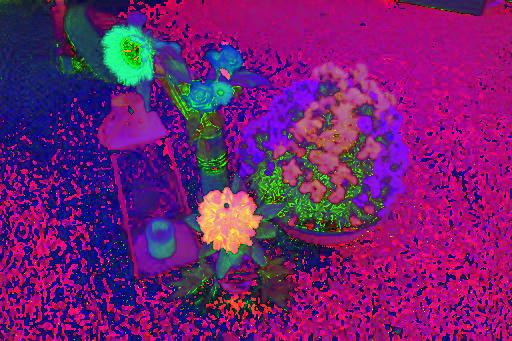
\includegraphics[width=\textwidth]{./figure/appendix/color_rep/images/imgHSI.jpg}
		\caption{}
		\label{fig:imgHSI}
    \end{subfigure}
    \begin{subfigure}[b]{0.49\textwidth}
        \centering
        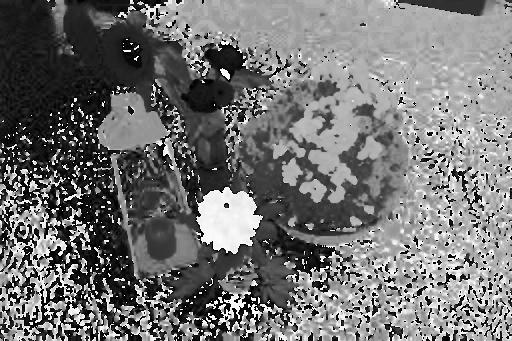
\includegraphics[width=\textwidth]{./figure/appendix/color_rep/images/imgH.jpg}
		\caption{}
		\label{fig:imgH}
    \end{subfigure}
    \begin{subfigure}[b]{0.49\textwidth}
        \centering
        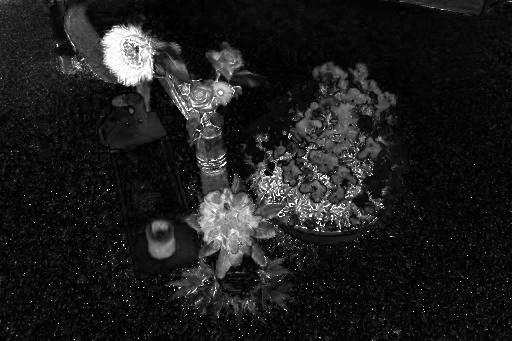
\includegraphics[width=\textwidth]{./figure/appendix/color_rep/images/imgS.jpg}
		\caption{}
		\label{fig:imgS}
    \end{subfigure}
    \begin{subfigure}[b]{0.49\textwidth}
        \centering
        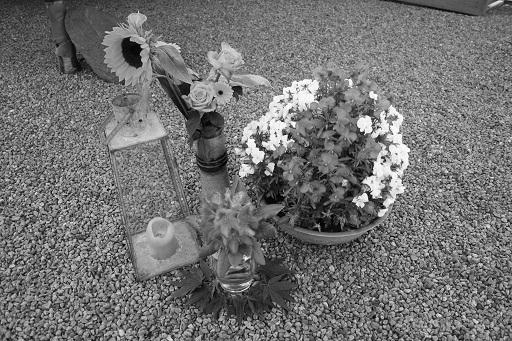
\includegraphics[width=\textwidth]{./figure/appendix/color_rep/images/imgI.jpg}
		\caption{}
		\label{fig:imgI}
    \end{subfigure}
    \caption{It is not evident from the \textbf{RGB} representation of the \textbf{HSI} color image shown in \textit{(a)} that the colors can be grouped based on one color channel, but is clearer from the Hue channel in \textit{(b)}, which shows large groupings for different parts of the image. The Saturation channels shows occasional grouping in \textit{(c)} but is not as uniform as the Hue, and the Intensity in \textit{(d)} shows large variations.}
    \label{fig:hsiChannels}
\end{figure}

\section{Color Indices using Near Infrared wavelengths}

One great thing with using electromagnetic radiation (light) as a source of information is that we do not need to use wavelengths comprehensible to our brains. The implications of this gives us the ability to use light information from wavelengths outside the visible spectrum. This can be of immense help when gathering information from biological living things which usually function in certain ways due to physical or chemical consequences. To further explain this we realise that light affect biological cells by exciting its building components to a higher energy state, and if the energy in a photon does not lie within the range of the possible excitation energies, there is no reason for a cell to absorb that light. So the reason why we cannot see certain wavelengths is due to almost full reflectance of those energies in our eyes receptors, and the same is true for most biological molecules as they are of the same order of magnitude in size and should be affected by roughly the same wavelengths, albeit in different ways. If we could somehow capture the near infra red light ($\lambda \approx \unit[750-1400]{nm}$) we could "see" the healthiness of a plant as a sick and degenerate cells does not behave as a living, healthy one as the molecules starts to crumble and behave differently.

\subsection{NDVI}

\textbf{NDVI} or \textbf{N}ormalized \textbf{D}ifference \textbf{V}egetation \textbf{I}ndex is used to differentiate healthy vegetation from either unhealthy or sparse vegetation  sections\cite{ndviSource}. What enables the usage of this index is that active chlorophyll in plants strongly absorbs visible light and a living cell strongly reflects near infrared light as it can not use this energy internally, and absorbing it would cause overheating. On the other hand, inactive or dead chlorophyll does not absorb the visible light to the same degree whereas the cell reflects roughly the same amount of near infrared light even if the chlorophyll is degenerate. The index is calculated by the formula,

\begin{equation}
	\label{eq:ndvi}
	NDVI = \frac{nR-VIS}{nR+VIS},
\end{equation}

where $nR$ is the near infrared index and $VIS$ is the representation of the visible light. This index ranges from -1 to +1 where a number close to +1 represents a healthy plant. Besides determining the health of plants, this index can also be used to determine what part of an image is a plant or not as a low index corresponds to sparse or no vegetation.

\subsection{SAVI}

The previously discussed index, \textbf{NDVI}, is great when determining the health of vegetation that is dense. If, on the other hand, the vegetations is sparse, then the reflectance of the soil could come to matter. Thus a \textbf{S}oil-\textbf{A}djusted \textbf{V}egetation \textbf{I}ndex \cite{saviSource}, \textbf{SAVI}, could help with this problem which is a modification of \textbf{NDVI} using a \textit{Soil brightness correction factor}, $L$ is introduced to and extends Eq.~\eqref{eq:ndvi} to,

\begin{equation}
	\label{eq:savi}
	SAVI=\frac{nR-VIS}{nR+VIS+L}(1+L),
\end{equation}

where $SAVI(L=0)=NDVI$. The factor $L$ is adjusted by the amount of green vegetation, where $L=1$ means a low amount of greenness and $L=0$ a large amount.

\subsection{MSAVI}

The biggest problem with the \textbf{SAVI} index is the parameter $L$ which is determined for each problem by trial-and-error. The \textbf{M}odified \textbf{S}oil-\textbf{A}djusted \textbf{V}egetation \textbf{I}ndex \cite{msaviSource}, \textbf{MSAVI} is calculated the same way as \textbf{SAVI} Eq.~\eqref{eq:savi},

\begin{equation}
    MSAVI = \frac{nR-VIS}{nR+VIS+L}(1+L),
\end{equation}

only that in this case, $L$ is not a constant but is calculated using,

\begin{equation}
	L = 1-\frac{2s\cdot(nR-VIS)(nR-s\cdot VIS)}{nR + VIS},
\end{equation}

where $s$ is yet another parameter, but is a equipment dependent parameter rather than application dependent one.

\subsection{MSAVI2}

The final Color index we will consider using the near infrared channel is completely parameter free, but the expression looks nastier. This new index is derived from \textbf{MSAVI} using recursion (the details will not be given here) and the final expression is calculated by,

\begin{equation}
    MSAVI2 = \frac{\left(2nR+1-\sqrt{\left(2nR+1\right)^2-8\left(nR-VIS\right)}\right)}{2}.
\end{equation}

\todv{Use the indices for healthy and unhealthy plants,
make new figure showing the comparisons}

These four color indices can be seen in \Cref{fig:rgbVSnrgbNDVI,fig:rgbVSnrgbSAVI,fig:rgbVSnrgbMSAVI,fig:rgbVSnrgbMSAVI2}.

\section{nRGB to RGB}

Above it is mentioned that near infrared light can come to help in various image analysis problems. However, this does not come for free, unless having access to really special equipment, most image light sensors only provide three different channels for capturing. Thus, the inclusion of a new channel, near infrared, implies the exclusion of another. The simplest would be to change it with the red channel as it lies closest in wavelength. If viewed using the \textbf{RGB} format, the resulting image will most likely be very reddish in color as most materials reflect the near infrared light, the comparison can be seen in \Cref{fig:rgbVSnrgb1,fig:rgbVSnrgb2}


\todv{Use this image to show rgb and nrgb channels}
\begin{figure}[H]
    \centering
    \captionsetup[subfigure]{justification=centering}
    \begin{subfigure}[b]{0.49\textwidth}
        \centering
        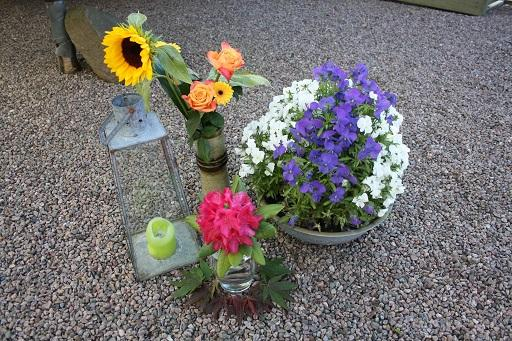
\includegraphics[width=\textwidth]{./figure/appendix/color_rep/images/imgRGB.jpg}
		\caption{}
		\label{fig:rgbVSnrgb1}
    \end{subfigure}
    \begin{subfigure}[b]{0.49\textwidth}
        \centering
        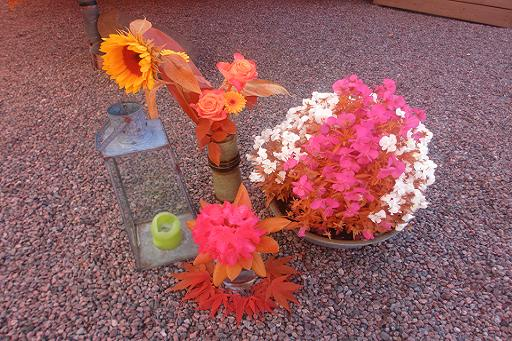
\includegraphics[width=\textwidth]{./figure/appendix/color_rep/images/nrgb.jpg}
		\caption{}
		\label{fig:rgbVSnrgb2}
    \end{subfigure}
    \begin{subfigure}[b]{0.49\textwidth}
        \centering
        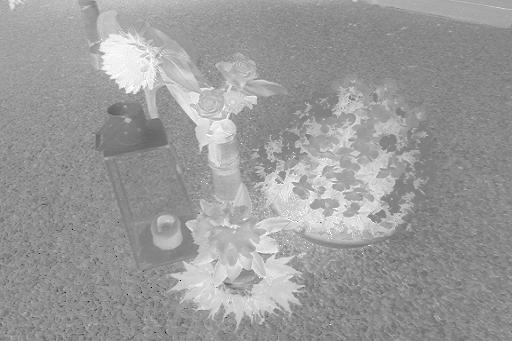
\includegraphics[width=\textwidth]{./figure/appendix/color_rep/images/ndvi.jpg}
		\caption{}
		\label{fig:rgbVSnrgbNDVI}
    \end{subfigure}
    \begin{subfigure}[b]{0.49\textwidth}
        \centering
        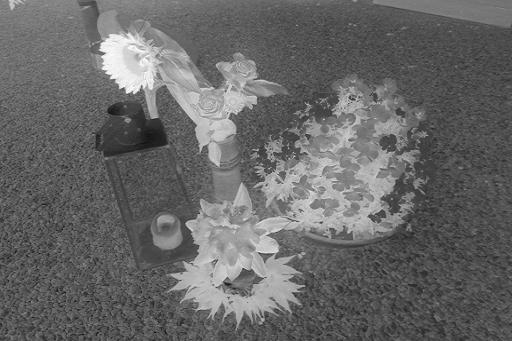
\includegraphics[width=\textwidth]{./figure/appendix/color_rep/images/savi.jpg}
		\caption{}
		\label{fig:rgbVSnrgbSAVI}
    \end{subfigure}
    \begin{subfigure}[b]{0.49\textwidth}
        \centering
        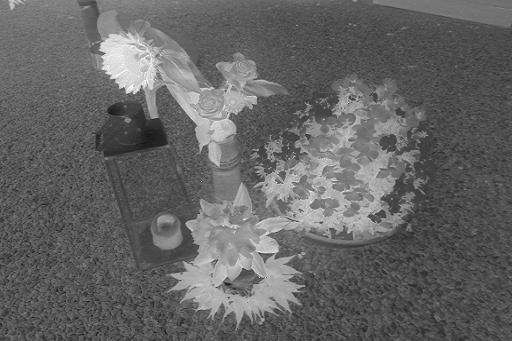
\includegraphics[width=\textwidth]{./figure/appendix/color_rep/images/msavi.jpg}
		\caption{}
		\label{fig:rgbVSnrgbMSAVI}
    \end{subfigure}
    \begin{subfigure}[b]{0.49\textwidth}
        \centering
        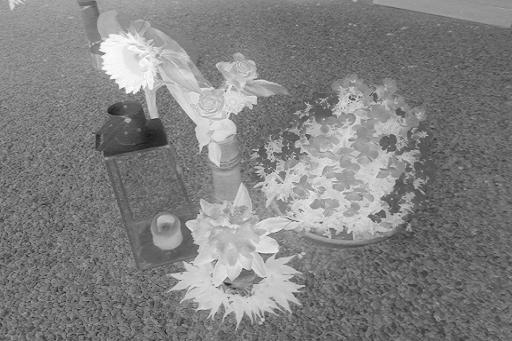
\includegraphics[width=\textwidth]{./figure/appendix/color_rep/images/msavi2.jpg}
		\caption{}
		\label{fig:rgbVSnrgbMSAVI2}
    \end{subfigure}
    \caption{}
    \label{fig:rgbVSnrgb}
\end{figure}

In order to show the \textbf{nRGB} image we want to "simulate" it as it was an ordinary \textbf{RGB} image. So we want to move the wavelengths of the new channel to a targeted one. Mathematically this is done using a convolution, described in Chapter.~\label{chap:conv}, with convolving function, $\delta(x)$ where $x$ is the targeted channels mean. This modification, replacing the red channel with the near infrared channel can be seen in Figure.~\ref{fig:fig:nRGBtoRGBmod}.

\begin{figure}[H]
    \centering
    \captionsetup[subfigure]{justification=centering}
    \begin{subfigure}[b]{0.49\textwidth}
        \centering
        \resizebox{\textwidth}{!}{
            % This file was created by matlab2tikz.
%
%The latest updates can be retrieved from
%  http://www.mathworks.com/matlabcentral/fileexchange/22022-matlab2tikz-matlab2tikz
%where you can also make suggestions and rate matlab2tikz.
%
\begin{tikzpicture}

\begin{axis}[%
width=4.521in,
height=3.53in,
at={(0.758in,0.517in)},
scale only axis,
xmin=390,
xmax=850,
xlabel={Wavelength, $\lambda\;[nm]$},
ymin=0,
ymax=1,
ytick={\empty},
ylabel={Intensity, $I$},
axis background/.style={fill=white},
title style={font=\bfseries},
title={Intensity ranges for nRGB color channels},
legend style={at={(0.97,0.03)},anchor=south east,legend cell align=left,align=left,draw=white!15!black}
]
\addplot [color=blue,dashdotted]
  table[row sep=crcr]{%
390	0\\
391	4.07641293463662e-07\\
392	6.37175299352561e-06\\
393	3.15068671549313e-05\\
394	9.72435132307244e-05\\
395	0.000231803023544704\\
396	0.000469222789545911\\
397	0.000848431011784255\\
398	0.00141236998654636\\
399	0.00220716697209077\\
400	0.00328135167742148\\
401	0.00468511941653912\\
402	0.00646963897110858\\
403	0.0086864042044825\\
404	0.0113866284700194\\
405	0.0146206808566358\\
406	0.0184375633145313\\
407	0.0228844277040258\\
408	0.0280061318104477\\
409	0.0338448333680121\\
410	0.0404396211356295\\
411	0.047826182067582\\
412	0.0560365036220067\\
413	0.0650986102501267\\
414	0.0750363331091675\\
415	0.0858691120418978\\
416	0.0976118288657348\\
417	0.110274671014352\\
418	0.12386302457473\\
419	0.138377395762587\\
420	0.153813359879131\\
421	0.170161536792071\\
422	0.187407591983826\\
423	0.205532262209874\\
424	0.224511404810172\\
425	0.244316069716601\\
426	0.264912593199353\\
427	0.286262712395227\\
428	0.308323699660747\\
429	0.331048515793055\\
430	0.354385981161518\\
431	0.37828096379298\\
432	0.40267458345361\\
433	0.427504430770273\\
434	0.452704800434371\\
435	0.478206937531092\\
436	0.503939296037\\
437	0.529827808528918\\
438	0.555796166147025\\
439	0.581766107855124\\
440	0.607657718041012\\
441	0.633389731499878\\
442	0.658879844843709\\
443	0.684045033379583\\
444	0.708801872499845\\
445	0.733066862627069\\
446	0.756756756756757\\
447	0.779788889640723\\
448	0.802081507654077\\
449	0.823554098388778\\
450	0.84412771901667\\
451	0.863725322464952\\
452	0.882272080447028\\
453	0.899695702391651\\
454	0.915926749313333\\
455	0.930898941666932\\
456	0.944549460229374\\
457	0.956819239051439\\
458	0.967653249522547\\
459	0.977000774591503\\
460	0.984815672186114\\
461	0.991056626874631\\
462	0.995687388811958\\
463	0.998676999013557\\
464	1\\
465	0.999636630855092\\
466	0.997573005740522\\
467	0.993801274909959\\
468	0.988319767265562\\
469	0.98113311349981\\
470	0.972252348865616\\
471	0.961694994617654\\
472	0.949485117167833\\
473	0.935653363997875\\
474	0.920236975371912\\
475	0.903279770892061\\
476	0.884832109939905\\
477	0.864950825046829\\
478	0.843699127236133\\
479	0.821146482379881\\
480	0.797368457613413\\
481	0.77244653685046\\
482	0.746467904441805\\
483	0.719525196020432\\
484	0.691716215576085\\
485	0.6631436178022\\
486	0.633914554758133\\
487	0.60414028588963\\
488	0.573935750450468\\
489	0.543419101368225\\
490	0.512711199597101\\
491	0.481935068000731\\
492	0.451215303807943\\
493	0.420677448684378\\
494	0.390447315462937\\
495	0.360650270575969\\
496	0.331410471232154\\
497	0.302850056381022\\
498	0.275088290508031\\
499	0.248240659303162\\
500	0.22241791624596\\
501	0.197725079149963\\
502	0.174260375709451\\
503	0.152114137091465\\
504	0.131367638616035\\
505	0.11209188656754\\
506	0.0943463501801598\\
507	0.0781776378403416\\
508	0.0636181165492335\\
509	0.0506844736880133\\
510	0.0393762201290571\\
511	0.0296741337358864\\
512	0.0215386422948316\\
513	0.0149081449213515\\
514	0.00969727098394851\\
515	0.00579507558861736\\
516	0.00306317066676766\\
517	0.00133379070955866\\
518	0.000407792191585641\\
519	5.25857268568126e-05\\
520	0\\
};
\addlegendentry{Blue channel};

\addplot [color=green,solid]
  table[row sep=crcr]{%
480	0\\
481	0.00093223626623717\\
482	0.00367135604495638\\
483	0.00813198417422354\\
484	0.0142300899828436\\
485	0.0218829872903608\\
486	0.0310093344070584\\
487	0.0415291341339586\\
488	0.0533637337628231\\
489	0.0664358250761532\\
490	0.0806694443471871\\
491	0.0959899723399044\\
492	0.112324134309023\\
493	0.1296\\
494	0.147746983649032\\
495	0.166695843983054\\
496	0.18637868421974\\
497	0.206728952067505\\
498	0.2276814397255\\
499	0.249172283883617\\
500	0.271138965722488\\
501	0.293520310913483\\
502	0.31625648961871\\
503	0.339289016491019\\
504	0.362560750673997\\
505	0.386015895801968\\
506	0.409600000000001\\
507	0.433259955883898\\
508	0.456944000560205\\
509	0.480601715626204\\
510	0.504184027169917\\
511	0.527643205770106\\
512	0.550932866496271\\
513	0.574007968908652\\
514	0.596824817058226\\
515	0.619341059486712\\
516	0.641515689226567\\
517	0.663309043800987\\
518	0.684682805223906\\
519	0.7056\\
520	0.72602499912468\\
521	0.7459235180841\\
522	0.765262616855152\\
523	0.784010699905465\\
524	0.80213751619341\\
525	0.819614159168096\\
526	0.83641306676937\\
527	0.85250802142782\\
528	0.867874150064773\\
529	0.882487924092294\\
530	0.896327159413187\\
531	0.909371016420994\\
532	0.921600000000001\\
533	0.932995959525227\\
534	0.943542088862435\\
535	0.953222926368125\\
536	0.962024354889535\\
537	0.969933601764644\\
538	0.97693923882217\\
539	0.983031182381569\\
540	0.988200693253038\\
541	0.992440376737509\\
542	0.995744182626659\\
543	0.998107405202899\\
544	0.999526683239382\\
545	1\\
546	0.999526683239382\\
547	0.998107405202899\\
548	0.995744182626659\\
549	0.992440376737509\\
550	0.988200693253038\\
551	0.983031182381569\\
552	0.97693923882217\\
553	0.969933601764644\\
554	0.962024354889535\\
555	0.953222926368125\\
556	0.943542088862435\\
557	0.932995959525227\\
558	0.921600000000001\\
559	0.909371016420994\\
560	0.896327159413185\\
561	0.882487924092293\\
562	0.867874150064773\\
563	0.85250802142782\\
564	0.83641306676937\\
565	0.819614159168096\\
566	0.80213751619341\\
567	0.784010699905465\\
568	0.765262616855152\\
569	0.7459235180841\\
570	0.72602499912468\\
571	0.7056\\
572	0.684682805223906\\
573	0.663309043800987\\
574	0.641515689226567\\
575	0.619341059486712\\
576	0.596824817058226\\
577	0.574007968908652\\
578	0.550932866496271\\
579	0.527643205770106\\
580	0.504184027169917\\
581	0.480601715626204\\
582	0.456944000560205\\
583	0.433259955883898\\
584	0.409600000000001\\
585	0.386015895801968\\
586	0.362560750673997\\
587	0.33928901649102\\
588	0.316256489618712\\
589	0.293520310913484\\
590	0.27113896572249\\
591	0.249172283883619\\
592	0.227681439725501\\
593	0.206728952067503\\
594	0.186378684219739\\
595	0.166695843983053\\
596	0.147746983649031\\
597	0.129599999999999\\
598	0.112324134309022\\
599	0.0959899723399034\\
600	0.0806694443471862\\
601	0.0664358250761524\\
602	0.0533637337628231\\
603	0.0415291341339586\\
604	0.0310093344070584\\
605	0.0218829872903608\\
606	0.0142300899828436\\
607	0.00813198417422354\\
608	0.00367135604495638\\
609	0.00093223626623717\\
610	0\\
};
\addlegendentry{Green channel};

\addplot [color=black!50!red,dotted]
  table[row sep=crcr]{%
680	0\\
681	0.1780945674663\\
682	0.250465484023825\\
683	0.305050935091026\\
684	0.350281495691377\\
685	0.38944333884865\\
686	0.424232154760807\\
687	0.45566141029005\\
688	0.484395476228516\\
689	0.51089866541581\\
690	0.535511134757081\\
691	0.558491276437065\\
692	0.580041095823919\\
693	0.600322252506667\\
694	0.619466653176438\\
695	0.637583703505814\\
696	0.654765425171487\\
697	0.671090160630024\\
698	0.686625315585877\\
699	0.701429428728179\\
700	0.715553760528563\\
701	0.729043531361233\\
702	0.74193889940319\\
703	0.754275742386741\\
704	0.766086289398919\\
705	0.777399636569839\\
706	0.788242171804457\\
707	0.798637927503085\\
708	0.808608875712866\\
709	0.818175176842255\\
710	0.827355390607196\\
711	0.836166656023381\\
712	0.84462484584854\\
713	0.852744699795073\\
714	0.860539939993475\\
715	0.868023371530233\\
716	0.875206970366371\\
717	0.882101960531949\\
718	0.888718882163266\\
719	0.895067651685132\\
720	0.901157615226465\\
721	0.906997596183015\\
722	0.91259593769817\\
723	0.91796054071513\\
724	0.92309889815638\\
725	0.928018125705421\\
726	0.932724989598114\\
727	0.937225931774254\\
728	0.941527092692205\\
729	0.945634332069051\\
730	0.94955324777439\\
731	0.953289193076732\\
732	0.956847292416436\\
733	0.960232455857784\\
734	0.963449392354308\\
735	0.966502621945626\\
736	0.9693964869903\\
737	0.972135162527271\\
738	0.974722665848055\\
739	0.977162865352837\\
740	0.979459488755651\\
741	0.981616130696928\\
742	0.983636259815556\\
743	0.985523225327241\\
744	0.987280263151216\\
745	0.988910501623148\\
746	0.990416966828369\\
747	0.991802587586268\\
748	0.993070200113741\\
749	0.99422255239297\\
750	0.995262308266485\\
751	0.996192051280345\\
752	0.997014288294441\\
753	0.99773145287719\\
754	0.998345908500441\\
755	0.998859951549003\\
756	0.999275814158003\\
757	0.999595666890181\\
758	0.999821621264208\\
759	0.99995573214423\\
760	1\\
761	0.999956373046231\\
762	0.999826749269117\\
763	0.99961297834735\\
764	0.999316863474413\\
765	0.998940163088391\\
766	0.998484592515113\\
767	0.997951825529966\\
768	0.997343495843362\\
769	0.996661198514478\\
770	0.995906491297533\\
771	0.995080895924601\\
772	0.994185899328655\\
773	0.993222954810295\\
774	0.992193483151365\\
775	0.991098873678464\\
776	0.989940485279148\\
777	0.988719647373421\\
778	0.987437660842979\\
779	0.986095798920466\\
780	0.984695308040897\\
781	0.983237408657247\\
782	0.981723296022068\\
783	0.980154140936922\\
784	0.978531090471251\\
785	0.976855268652255\\
786	0.975127777127241\\
787	0.973349695799787\\
788	0.971522083441043\\
789	0.969645978277363\\
790	0.967722398555419\\
791	0.965752343085879\\
792	0.963736791766657\\
793	0.961676706086704\\
794	0.959573029611245\\
795	0.957426688449308\\
796	0.955238591704372\\
797	0.953009631908882\\
798	0.950740685443365\\
799	0.948432612940833\\
800	0.946086259677112\\
801	0.943702455947724\\
802	0.9412820174319\\
803	0.938825745544273\\
804	0.936334427774783\\
805	0.933808838017285\\
806	0.93124973688734\\
807	0.928657872029632\\
808	0.926033978415442\\
809	0.923378778630582\\
810	0.920692983154181\\
811	0.91797729062868\\
812	0.915232388121403\\
813	0.912458951378019\\
814	0.909657645068224\\
815	0.906829123023941\\
816	0.903974028470335\\
817	0.9010929942499\\
818	0.898186643039908\\
819	0.895255587563442\\
820	0.892300430794275\\
821	0.889321766155811\\
822	0.886320177714312\\
823	0.883296240366619\\
824	0.880250520022567\\
825	0.877183573782285\\
826	0.874095950108561\\
827	0.870988188994457\\
828	0.867860822126327\\
829	0.864714373042411\\
830	0.861549357287152\\
831	0.858366282561391\\
832	0.855165648868566\\
833	0.851947948657072\\
834	0.84871366695889\\
835	0.84546328152463\\
836	0.842197262955093\\
837	0.838916074829471\\
838	0.835620173830302\\
839	0.832310009865272\\
840	0.828986026185987\\
841	0.825648659503785\\
842	0.822298340102712\\
843	0.818935491949727\\
844	0.815560532802245\\
845	0.812173874313074\\
846	0.808775922132867\\
847	0.805367076010118\\
848	0.801947729888824\\
849	0.798518272003846\\
850	0.795079084974062\\
851	0.791630545893377\\
852	0.788173026419636\\
853	0.784706892861528\\
854	0.781232506263519\\
855	0.777750222488885\\
856	0.774260392300896\\
857	0.770763361442205\\
858	0.767259470712488\\
859	0.763749056044401\\
860	0.760232448577881\\
861	0.756709974732858\\
862	0.753181956280405\\
863	0.749648710412386\\
864	0.746110549809627\\
865	0.742567782708668\\
866	0.739020712967124\\
867	0.735469640127689\\
868	0.731914859480839\\
869	0.728356662126245\\
870	0.724795335032949\\
871	0.72123116109833\\
872	0.717664419205882\\
873	0.714095384281858\\
874	0.710524327350788\\
875	0.70695151558991\\
876	0.703377212382542\\
877	0.699801677370422\\
878	0.696225166505043\\
879	0.692647932098002\\
880	0.6890702228704\\
881	0.685492284001305\\
882	0.681914357175313\\
883	0.678336680629217\\
884	0.674759489197814\\
885	0.671183014358879\\
886	0.667607484277297\\
887	0.66403312384842\\
888	0.660460154740617\\
889	0.656888795437078\\
890	0.653319261276864\\
891	0.649751764495237\\
892	0.64618651426327\\
893	0.642623716726777\\
894	0.639063575044555\\
895	0.635506289425972\\
896	0.631952057167906\\
897	0.628401072691056\\
898	0.624853527575635\\
899	0.621309610596462\\
900	0.617769507757463\\
901	0.614233402325605\\
902	0.610701474864259\\
903	0.607173903266019\\
904	0.603650862784981\\
905	0.600132526068502\\
906	0.596619063188436\\
907	0.593110641671882\\
908	0.589607426531426\\
909	0.586109580294912\\
910	0.582617263034739\\
911	0.579130632396704\\
912	0.575649843628381\\
913	0.572175049607078\\
914	0.56870640086735\\
915	0.565244045628092\\
916	0.561788129819222\\
917	0.558338797107962\\
918	0.554896188924712\\
919	0.551460444488549\\
920	0.54803170083234\\
921	0.544610092827482\\
922	0.54119575320828\\
923	0.537788812595969\\
924	0.534389399522382\\
925	0.530997640453279\\
926	0.527613659811342\\
927	0.524237579998835\\
928	0.520869521419945\\
929	0.517509602502807\\
930	0.51415793972122\\
931	0.510814647616056\\
932	0.507479838816373\\
933	0.504153624060238\\
934	0.500836112215256\\
935	0.49752741029883\\
936	0.494227623498134\\
937	0.490936855189822\\
938	0.487655206959471\\
939	0.484382778620761\\
940	0.481119668234405\\
941	0.477865972126821\\
942	0.474621784908567\\
943	0.471387199492527\\
944	0.468162307111868\\
945	0.464947197337752\\
946	0.461741958096838\\
947	0.458546675688543\\
948	0.455361434802092\\
949	0.452186318533349\\
950	0.449021408401442\\
951	0.445866784365168\\
952	0.442722524839205\\
953	0.439588706710116\\
954	0.436465405352161\\
955	0.433352694642909\\
956	0.430250646978663\\
957	0.427159333289702\\
958	0.424078823055329\\
959	0.421009184318749\\
960	0.417950483701761\\
961	0.414902786419281\\
962	0.411866156293692\\
963	0.408840655769023\\
964	0.405826345924967\\
965	0.40282328649073\\
966	0.399831535858728\\
967	0.396851151098117\\
968	0.393882187968174\\
969	0.390924700931528\\
970	0.387978743167231\\
971	0.385044366583696\\
972	0.382121621831478\\
973	0.379210558315917\\
974	0.376311224209644\\
975	0.373423666464941\\
976	0.370547930825978\\
977	0.3676840618409\\
978	0.364832102873797\\
979	0.361992096116539\\
980	0.359164082600481\\
981	0.356348102208049\\
982	0.353544193684198\\
983	0.350752394647749\\
984	0.347972741602611\\
985	0.345205269948881\\
986	0.342450013993829\\
987	0.339707006962771\\
988	0.336976281009826\\
989	0.334257867228571\\
990	0.331551795662575\\
991	0.328858095315835\\
992	0.326176794163108\\
993	0.323507919160127\\
994	0.32085149625373\\
995	0.318207550391876\\
996	0.315576105533573\\
997	0.312957184658693\\
998	0.310350809777709\\
999	0.307757001941322\\
1000	0.30517578125\\
1001	0.302607166863431\\
1002	0.300051177009871\\
1003	0.297507828995419\\
1004	0.29497713921319\\
1005	0.292459123152407\\
1006	0.289953795407411\\
1007	0.287461169686581\\
1008	0.284981258821168\\
1009	0.282514074774061\\
1010	0.280059628648451\\
1011	0.277617930696438\\
1012	0.275188990327538\\
1013	0.272772816117132\\
1014	0.270369415814821\\
1015	0.267978796352722\\
1016	0.265600963853673\\
1017	0.26323592363938\\
1018	0.260883680238484\\
1019	0.258544237394554\\
1020	0.256217598074016\\
1021	0.253903764474012\\
1022	0.251602738030184\\
1023	0.249314519424399\\
1024	0.247039108592401\\
1025	0.244776504731404\\
1026	0.242526706307609\\
1027	0.240289711063671\\
1028	0.238065516026091\\
1029	0.235854117512555\\
1030	0.233655511139204\\
1031	0.231469691827846\\
1032	0.229296653813112\\
1033	0.227136390649549\\
1034	0.224988895218653\\
1035	0.222854159735849\\
1036	0.22073217575741\\
1037	0.218622934187326\\
1038	0.216526425284109\\
1039	0.21444263866755\\
1040	0.212371563325422\\
1041	0.210313187620122\\
1042	0.208267499295273\\
1043	0.206234485482264\\
1044	0.204214132706742\\
1045	0.202206426895051\\
1046	0.200211353380629\\
1047	0.198228896910344\\
1048	0.196259041650792\\
1049	0.19430177119454\\
1050	0.19235706856632\\
1051	0.190424916229186\\
1052	0.188505296090612\\
1053	0.186598189508554\\
1054	0.184703577297463\\
1055	0.182821439734248\\
1056	0.180951756564205\\
1057	0.179094507006897\\
1058	0.177249669761987\\
1059	0.175417223015036\\
1060	0.173597144443255\\
1061	0.171789411221212\\
1062	0.169994000026507\\
1063	0.168210887045395\\
1064	0.166440047978378\\
1065	0.164681458045756\\
1066	0.162935091993129\\
1067	0.161200924096876\\
1068	0.159478928169583\\
1069	0.157769077565436\\
1070	0.156071345185584\\
1071	0.154385703483453\\
1072	0.152712124470033\\
1073	0.151050579719123\\
1074	0.149401040372545\\
1075	0.147763477145316\\
1076	0.146137860330793\\
1077	0.144524159805778\\
1078	0.142922345035588\\
1079	0.141332385079096\\
1080	0.139754248593737\\
1081	0.138187903840476\\
1082	0.13663331868875\\
1083	0.135090460621373\\
1084	0.133559296739414\\
1085	0.132039793767035\\
1086	0.130531918056308\\
1087	0.129035635591992\\
1088	0.127550911996285\\
1089	0.126077712533546\\
1090	0.124616002114979\\
1091	0.123165745303299\\
1092	0.121726906317362\\
1093	0.120299449036765\\
1094	0.11888333700642\\
1095	0.117478533441101\\
1096	0.116085001229957\\
1097	0.114702702941004\\
1098	0.113331600825585\\
1099	0.111971656822807\\
1100	0.110622832563944\\
1101	0.109285089376819\\
1102	0.107958388290161\\
1103	0.106642690037932\\
1104	0.105337955063626\\
1105	0.104044143524549\\
1106	0.102761215296071\\
1107	0.101489129975851\\
1108	0.100227846888038\\
1109	0.0989773250874479\\
1110	0.0977375233637198\\
1111	0.0965084002454404\\
1112	0.0952899140042508\\
1113	0.0940820226589277\\
1114	0.0928846839794414\\
1115	0.0916978554909906\\
1116	0.0905214944780144\\
1117	0.0893555579881817\\
1118	0.0882000028363584\\
1119	0.0870547856085516\\
1120	0.085919862665833\\
1121	0.0847951901482393\\
1122	0.0836807239786523\\
1123	0.0825764198666566\\
1124	0.0814822333123765\\
1125	0.0803981196102924\\
1126	0.0793240338530359\\
1127	0.0782599309351644\\
1128	0.0772057655569162\\
1129	0.0761614922279439\\
1130	0.0751270652710294\\
1131	0.0741024388257785\\
1132	0.0730875668522957\\
1133	0.0720824031348397\\
1134	0.0710869012854604\\
1135	0.0701010147476158\\
1136	0.0691246967997708\\
1137	0.0681579005589775\\
1138	0.0672005789844357\\
1139	0.0662526848810369\\
1140	0.0653141709028885\\
1141	0.0643849895568217\\
1142	0.0634650932058796\\
1143	0.0625544340727895\\
1144	0.0616529642434165\\
1145	0.0607606356702003\\
1146	0.0598774001755744\\
1147	0.0590032094553691\\
1148	0.0581380150821967\\
1149	0.0572817685088205\\
1150	0.0564344210715071\\
1151	0.0555959239933623\\
1152	0.0547662283876508\\
1153	0.0539452852610995\\
1154	0.0531330455171856\\
1155	0.0523294599594074\\
1156	0.0515344792945412\\
1157	0.0507480541358811\\
1158	0.0499701350064643\\
1159	0.0492006723422809\\
1160	0.0484396164954682\\
1161	0.0476869177374904\\
1162	0.0469425262623033\\
1163	0.0462063921895043\\
1164	0.0454784655674672\\
1165	0.0447586963764636\\
1166	0.0440470345317687\\
1167	0.0433434298867538\\
1168	0.042647832235964\\
1169	0.0419601913181824\\
1170	0.0412804568194799\\
1171	0.0406085783762516\\
1172	0.0399445055782396\\
1173	0.0392881879715417\\
1174	0.0386395750616072\\
1175	0.0379986163162192\\
1176	0.0373652611684637\\
1177	0.0367394590196856\\
1178	0.0361211592424316\\
1179	0.0355103111833803\\
1180	0.0349068641662597\\
1181	0.034310767494752\\
1182	0.0337219704553849\\
1183	0.0331404223204123\\
1184	0.0325660723506808\\
1185	0.0319988697984849\\
1186	0.03143876391041\\
1187	0.030885703930163\\
1188	0.0303396391013911\\
1189	0.0298005186704888\\
1190	0.0292682918893932\\
1191	0.0287429080183673\\
1192	0.0282243163287716\\
1193	0.0277124661058252\\
1194	0.0272073066513542\\
1195	0.0267087872865298\\
1196	0.0262168573545944\\
1197	0.0257314662235771\\
1198	0.025252563288998\\
1199	0.0247800979765614\\
1200	0.0243140197448386\\
1201	0.0238542780879391\\
1202	0.0234008225381717\\
1203	0.022953602668695\\
1204	0.0225125680961571\\
1205	0.0220776684833247\\
1206	0.0216488535417025\\
1207	0.0212260730341414\\
1208	0.0208092767774375\\
1209	0.0203984146449198\\
1210	0.0199934365690286\\
1211	0.0195942925438842\\
1212	0.0192009326278446\\
1213	0.0188133069460544\\
1214	0.0184313656929835\\
1215	0.018055059134956\\
1216	0.0176843376126697\\
1217	0.0173191515437062\\
1218	0.0169594514250309\\
1219	0.0166051878354843\\
1220	0.016256311438264\\
1221	0.0159127729833964\\
1222	0.0155745233102004\\
1223	0.0152415133497416\\
1224	0.0149136941272769\\
1225	0.014591016764691\\
1226	0.0142734324829233\\
1227	0.0139608926043863\\
1228	0.0136533485553749\\
1229	0.0133507518684672\\
1230	0.0130530541849165\\
1231	0.012760207257035\\
1232	0.0124721629505686\\
1233	0.0121888732470629\\
1234	0.0119102902462221\\
1235	0.0116363661682577\\
1236	0.0113670533562303\\
1237	0.0111023042783828\\
1238	0.0108420715304651\\
1239	0.0105863078380508\\
1240	0.0103349660588461\\
1241	0.0100879991849903\\
1242	0.00984536034534893\\
1243	0.00960700280779797\\
1244	0.00937287998150131\\
1245	0.00914294541917976\\
1246	0.00891715281937253\\
1247	0.00869545602869099\\
1248	0.00847780904406483\\
1249	0.00826416601498059\\
1250	0.00805448124571272\\
1251	0.00784870919754711\\
1252	0.00764680449099724\\
1253	0.00744872190801294\\
1254	0.00725441639418183\\
1255	0.00706384306092347\\
1256	0.00687695718767632\\
1257	0.00669371422407748\\
1258	0.00651406979213539\\
1259	0.0063379796883953\\
1260	0.00616539988609789\\
1261	0.00599628653733076\\
1262	0.00583059597517305\\
1263	0.00566828471583319\\
1264	0.00550930946077972\\
1265	0.00535362709886542\\
1266	0.0052011947084446\\
1267	0.00505196955948369\\
1268	0.00490590911566522\\
1269	0.00476297103648511\\
1270	0.00462311317934347\\
1271	0.00448629360162872\\
1272	0.00435247056279533\\
1273	0.00422160252643514\\
1274	0.00409364816234212\\
1275	0.00396856634857093\\
1276	0.00384631617348903\\
1277	0.00372685693782258\\
1278	0.00361014815669604\\
1279	0.0034961495616656\\
1280	0.00338482110274646\\
1281	0.00327612295043391\\
1282	0.0031700154977184\\
1283	0.00306645936209452\\
1284	0.00296541538756399\\
1285	0.00286684464663267\\
1286	0.00277070844230161\\
1287	0.00267696831005223\\
1288	0.00258558601982567\\
1289	0.00249652357799623\\
1290	0.0024097432293391\\
1291	0.00232520745899231\\
1292	0.00224287899441293\\
1293	0.00216272080732769\\
1294	0.00208469611567782\\
1295	0.0020087683855584\\
1296	0.00193490133315204\\
1297	0.00186305892665708\\
1298	0.00179320538821027\\
1299	0.00172530519580395\\
1300	0.00165932308519782\\
1301	0.00159522405182526\\
1302	0.00153297335269435\\
1303	0.00147253650828346\\
1304	0.00141387930443161\\
1305	0.00135696779422346\\
1306	0.00130176829986916\\
1307	0.00124824741457888\\
1308	0.00119637200443228\\
1309	0.00114610921024266\\
1310	0.00109742644941616\\
1311	0.00105029141780575\\
1312	0.00100467209156021\\
1313	0.000960536728968084\\
1314	0.000917853872296571\\
1315	0.000876592349625543\\
1316	0.000836721276676519\\
1317	0.000798210058636791\\
1318	0.00076102839197864\\
1319	0.0007251462662737\\
1320	0.000690533966002486\\
1321	0.000657162072359132\\
1322	0.000625001465051347\\
1323	0.000594023324095629\\
1324	0.000564199131607762\\
1325	0.000535500673588623\\
1326	0.000507900041705318\\
1327	0.000481369635067687\\
1328	0.000455882162000201\\
1329	0.000431410641809266\\
1330	0.000407928406545971\\
1331	0.000385409102764312\\
1332	0.000363826693274897\\
1333	0.000343155458894175\\
1334	0.00032337000018921\\
1335	0.000304445239218023\\
1336	0.000286356421265527\\
1337	0.00026907911657508\\
1338	0.000252589222075679\\
1339	0.00023686296310483\\
1340	0.000221876895127097\\
1341	0.000207607905448375\\
1342	0.000194033214925899\\
1343	0.000181130379674014\\
1344	0.000168877292765733\\
1345	0.000157252185930103\\
1346	0.000146233631245404\\
1347	0.000135800542828201\\
1348	0.000125932178518275\\
1349	0.000116608141559451\\
1350	0.000107808382276355\\
1351	9.95131997471056e-05\\
1352	9.17032434719806e-05\\
1353	8.43595150380666e-05\\
1354	7.74633697799207e-05\\
1355	7.09965184362616e-05\\
1356	6.49410288027146e-05\\
1357	5.927932738063e-05\\
1358	5.39942010219941e-05\\
1359	4.90687985704616e-05\\
1360	4.44866324985143e-05\\
1361	4.02315805407853e-05\\
1362	3.62878873235561e-05\\
1363	3.26401659904515e-05\\
1364	2.92733998243521e-05\\
1365	2.61729438655429e-05\\
1366	2.33245265261204e-05\\
1367	2.07142512006748e-05\\
1368	1.83285978732689e-05\\
1369	1.61544247207321e-05\\
1370	1.41789697122891e-05\\
1371	1.23898522055416e-05\\
1372	1.07750745388233e-05\\
1373	9.32302361994526e-06\\
1374	8.0224725113513e-06\\
1375	6.86258201170222e-06\\
1376	5.83290223390606e-06\\
1377	4.92337417961355e-06\\
1378	4.12433131019649e-06\\
1379	3.42650111422712e-06\\
1380	2.82100667147619e-06\\
1381	2.29936821344752e-06\\
1382	1.85350468046667e-06\\
1383	1.47573527534102e-06\\
1384	1.1587810136087e-06\\
1385	8.95766270393578e-07\\
1386	6.80220323883226e-07\\
1387	5.06078895447043e-07\\
1388	3.67685686411175e-07\\
1389	2.59793911507053e-07\\
1390	1.77567829010087e-07\\
1391	1.16584267585038e-07\\
1392	7.28341498543783e-08\\
1393	4.27240127059308e-08\\
1394	2.3077524355879e-08\\
1395	1.1136998183189e-08\\
1396	4.5649033513344e-09\\
1397	1.44537223312122e-09\\
1398	2.85704654292057e-10\\
1399	1.7868971483619e-11\\
1400	7.30083046639805e-64\\
};
\addlegendentry{Near infrared channel};

\end{axis}
\end{tikzpicture}%

        }
		\caption{}
    \end{subfigure}
    \begin{subfigure}[b]{0.49\textwidth}
        \centering
        \resizebox{\textwidth}{!}{
            % This file was created by matlab2tikz.
%
%The latest updates can be retrieved from
%  http://www.mathworks.com/matlabcentral/fileexchange/22022-matlab2tikz-matlab2tikz
%where you can also make suggestions and rate matlab2tikz.
%
\begin{tikzpicture}

\begin{axis}[%
width=4.521in,
height=3.53in,
at={(0.758in,0.517in)},
scale only axis,
xmin=390,
xmax=850,
xlabel={Wavelength, $\lambda\;[nm]$},
ymin=0,
ymax=1,
ytick={\empty},
ylabel={Intensity, $I$},
axis background/.style={fill=white},
title style={font=\bfseries},
title={Intensity ranges for modified nRGB color channels},
legend style={at={(0.97,0.03)},anchor=south east,legend cell align=left,align=left,draw=white!15!black}
]
\addplot [color=blue,dashdotted]
  table[row sep=crcr]{%
390	0\\
391	4.07641293463662e-07\\
392	6.37175299352561e-06\\
393	3.15068671549313e-05\\
394	9.72435132307244e-05\\
395	0.000231803023544704\\
396	0.000469222789545911\\
397	0.000848431011784255\\
398	0.00141236998654636\\
399	0.00220716697209077\\
400	0.00328135167742148\\
401	0.00468511941653912\\
402	0.00646963897110858\\
403	0.0086864042044825\\
404	0.0113866284700194\\
405	0.0146206808566358\\
406	0.0184375633145313\\
407	0.0228844277040258\\
408	0.0280061318104477\\
409	0.0338448333680121\\
410	0.0404396211356295\\
411	0.047826182067582\\
412	0.0560365036220067\\
413	0.0650986102501267\\
414	0.0750363331091675\\
415	0.0858691120418978\\
416	0.0976118288657348\\
417	0.110274671014352\\
418	0.12386302457473\\
419	0.138377395762587\\
420	0.153813359879131\\
421	0.170161536792071\\
422	0.187407591983826\\
423	0.205532262209874\\
424	0.224511404810172\\
425	0.244316069716601\\
426	0.264912593199353\\
427	0.286262712395227\\
428	0.308323699660747\\
429	0.331048515793055\\
430	0.354385981161518\\
431	0.37828096379298\\
432	0.40267458345361\\
433	0.427504430770273\\
434	0.452704800434371\\
435	0.478206937531092\\
436	0.503939296037\\
437	0.529827808528918\\
438	0.555796166147025\\
439	0.581766107855124\\
440	0.607657718041012\\
441	0.633389731499878\\
442	0.658879844843709\\
443	0.684045033379583\\
444	0.708801872499845\\
445	0.733066862627069\\
446	0.756756756756757\\
447	0.779788889640723\\
448	0.802081507654077\\
449	0.823554098388778\\
450	0.84412771901667\\
451	0.863725322464952\\
452	0.882272080447028\\
453	0.899695702391651\\
454	0.915926749313333\\
455	0.930898941666932\\
456	0.944549460229374\\
457	0.956819239051439\\
458	0.967653249522547\\
459	0.977000774591503\\
460	0.984815672186114\\
461	0.991056626874631\\
462	0.995687388811958\\
463	0.998676999013557\\
464	1\\
465	0.999636630855092\\
466	0.997573005740522\\
467	0.993801274909959\\
468	0.988319767265562\\
469	0.98113311349981\\
470	0.972252348865616\\
471	0.961694994617654\\
472	0.949485117167833\\
473	0.935653363997875\\
474	0.920236975371912\\
475	0.903279770892061\\
476	0.884832109939905\\
477	0.864950825046829\\
478	0.843699127236133\\
479	0.821146482379881\\
480	0.797368457613413\\
481	0.77244653685046\\
482	0.746467904441805\\
483	0.719525196020432\\
484	0.691716215576085\\
485	0.6631436178022\\
486	0.633914554758133\\
487	0.60414028588963\\
488	0.573935750450468\\
489	0.543419101368225\\
490	0.512711199597101\\
491	0.481935068000731\\
492	0.451215303807943\\
493	0.420677448684378\\
494	0.390447315462937\\
495	0.360650270575969\\
496	0.331410471232154\\
497	0.302850056381022\\
498	0.275088290508031\\
499	0.248240659303162\\
500	0.22241791624596\\
501	0.197725079149963\\
502	0.174260375709451\\
503	0.152114137091465\\
504	0.131367638616035\\
505	0.11209188656754\\
506	0.0943463501801598\\
507	0.0781776378403416\\
508	0.0636181165492335\\
509	0.0506844736880133\\
510	0.0393762201290571\\
511	0.0296741337358864\\
512	0.0215386422948316\\
513	0.0149081449213515\\
514	0.00969727098394851\\
515	0.00579507558861736\\
516	0.00306317066676766\\
517	0.00133379070955866\\
518	0.000407792191585641\\
519	5.25857268568126e-05\\
520	0\\
};
\addlegendentry{Blue channel};

\addplot [color=green,solid]
  table[row sep=crcr]{%
480	0\\
481	0.00093223626623717\\
482	0.00367135604495638\\
483	0.00813198417422354\\
484	0.0142300899828436\\
485	0.0218829872903608\\
486	0.0310093344070584\\
487	0.0415291341339586\\
488	0.0533637337628231\\
489	0.0664358250761532\\
490	0.0806694443471871\\
491	0.0959899723399044\\
492	0.112324134309023\\
493	0.1296\\
494	0.147746983649032\\
495	0.166695843983054\\
496	0.18637868421974\\
497	0.206728952067505\\
498	0.2276814397255\\
499	0.249172283883617\\
500	0.271138965722488\\
501	0.293520310913483\\
502	0.31625648961871\\
503	0.339289016491019\\
504	0.362560750673997\\
505	0.386015895801968\\
506	0.409600000000001\\
507	0.433259955883898\\
508	0.456944000560205\\
509	0.480601715626204\\
510	0.504184027169917\\
511	0.527643205770106\\
512	0.550932866496271\\
513	0.574007968908652\\
514	0.596824817058226\\
515	0.619341059486712\\
516	0.641515689226567\\
517	0.663309043800987\\
518	0.684682805223906\\
519	0.7056\\
520	0.72602499912468\\
521	0.7459235180841\\
522	0.765262616855152\\
523	0.784010699905465\\
524	0.80213751619341\\
525	0.819614159168096\\
526	0.83641306676937\\
527	0.85250802142782\\
528	0.867874150064773\\
529	0.882487924092294\\
530	0.896327159413187\\
531	0.909371016420994\\
532	0.921600000000001\\
533	0.932995959525227\\
534	0.943542088862435\\
535	0.953222926368125\\
536	0.962024354889535\\
537	0.969933601764644\\
538	0.97693923882217\\
539	0.983031182381569\\
540	0.988200693253038\\
541	0.992440376737509\\
542	0.995744182626659\\
543	0.998107405202899\\
544	0.999526683239382\\
545	1\\
546	0.999526683239382\\
547	0.998107405202899\\
548	0.995744182626659\\
549	0.992440376737509\\
550	0.988200693253038\\
551	0.983031182381569\\
552	0.97693923882217\\
553	0.969933601764644\\
554	0.962024354889535\\
555	0.953222926368125\\
556	0.943542088862435\\
557	0.932995959525227\\
558	0.921600000000001\\
559	0.909371016420994\\
560	0.896327159413185\\
561	0.882487924092293\\
562	0.867874150064773\\
563	0.85250802142782\\
564	0.83641306676937\\
565	0.819614159168096\\
566	0.80213751619341\\
567	0.784010699905465\\
568	0.765262616855152\\
569	0.7459235180841\\
570	0.72602499912468\\
571	0.7056\\
572	0.684682805223906\\
573	0.663309043800987\\
574	0.641515689226567\\
575	0.619341059486712\\
576	0.596824817058226\\
577	0.574007968908652\\
578	0.550932866496271\\
579	0.527643205770106\\
580	0.504184027169917\\
581	0.480601715626204\\
582	0.456944000560205\\
583	0.433259955883898\\
584	0.409600000000001\\
585	0.386015895801968\\
586	0.362560750673997\\
587	0.33928901649102\\
588	0.316256489618712\\
589	0.293520310913484\\
590	0.27113896572249\\
591	0.249172283883619\\
592	0.227681439725501\\
593	0.206728952067503\\
594	0.186378684219739\\
595	0.166695843983053\\
596	0.147746983649031\\
597	0.129599999999999\\
598	0.112324134309022\\
599	0.0959899723399034\\
600	0.0806694443471862\\
601	0.0664358250761524\\
602	0.0533637337628231\\
603	0.0415291341339586\\
604	0.0310093344070584\\
605	0.0218829872903608\\
606	0.0142300899828436\\
607	0.00813198417422354\\
608	0.00367135604495638\\
609	0.00093223626623717\\
610	0\\
};
\addlegendentry{Green channel};

\addplot [color=black!50!red,dotted]
  table[row sep=crcr]{%
580	0\\
581	0.1780945674663\\
582	0.250465484023825\\
583	0.305050935091026\\
584	0.350281495691377\\
585	0.38944333884865\\
586	0.424232154760807\\
587	0.45566141029005\\
588	0.484395476228516\\
589	0.51089866541581\\
590	0.535511134757083\\
591	0.558491276437067\\
592	0.580041095823921\\
593	0.600322252506669\\
594	0.619466653176439\\
595	0.637583703505816\\
596	0.654765425171489\\
597	0.671090160630025\\
598	0.686625315585878\\
599	0.70142942872818\\
600	0.715553760528565\\
601	0.729043531361234\\
602	0.74193889940319\\
603	0.754275742386741\\
604	0.766086289398919\\
605	0.777399636569839\\
606	0.788242171804457\\
607	0.798637927503085\\
608	0.808608875712866\\
609	0.818175176842255\\
610	0.827355390607196\\
611	0.836166656023381\\
612	0.84462484584854\\
613	0.852744699795073\\
614	0.860539939993476\\
615	0.868023371530233\\
616	0.875206970366371\\
617	0.88210196053195\\
618	0.888718882163266\\
619	0.895067651685132\\
620	0.901157615226466\\
621	0.906997596183015\\
622	0.91259593769817\\
623	0.917960540715131\\
624	0.92309889815638\\
625	0.928018125705421\\
626	0.932724989598115\\
627	0.937225931774255\\
628	0.941527092692206\\
629	0.945634332069051\\
630	0.949553247774391\\
631	0.953289193076732\\
632	0.956847292416436\\
633	0.960232455857785\\
634	0.963449392354308\\
635	0.966502621945626\\
636	0.9693964869903\\
637	0.972135162527271\\
638	0.974722665848055\\
639	0.977162865352837\\
640	0.979459488755651\\
641	0.981616130696928\\
642	0.983636259815556\\
643	0.985523225327241\\
644	0.987280263151216\\
645	0.988910501623148\\
646	0.990416966828369\\
647	0.991802587586268\\
648	0.993070200113741\\
649	0.99422255239297\\
650	0.995262308266485\\
651	0.996192051280345\\
652	0.997014288294441\\
653	0.99773145287719\\
654	0.998345908500441\\
655	0.998859951549003\\
656	0.999275814158003\\
657	0.999595666890181\\
658	0.999821621264208\\
659	0.99995573214423\\
660	1\\
661	0.999956373046231\\
662	0.999826749269117\\
663	0.99961297834735\\
664	0.999316863474413\\
665	0.998940163088391\\
666	0.998484592515113\\
667	0.997951825529966\\
668	0.997343495843362\\
669	0.996661198514478\\
670	0.995906491297533\\
671	0.9950808959246\\
672	0.994185899328655\\
673	0.993222954810295\\
674	0.992193483151365\\
675	0.991098873678464\\
676	0.989940485279148\\
677	0.988719647373421\\
678	0.987437660842979\\
679	0.986095798920465\\
680	0.984695308040897\\
681	0.983237408657247\\
682	0.981723296022068\\
683	0.980154140936922\\
684	0.978531090471251\\
685	0.976855268652255\\
686	0.975127777127241\\
687	0.973349695799787\\
688	0.971522083441043\\
689	0.969645978277363\\
690	0.967722398555419\\
691	0.965752343085879\\
692	0.963736791766657\\
693	0.961676706086704\\
694	0.959573029611245\\
695	0.957426688449308\\
696	0.955238591704372\\
697	0.953009631908882\\
698	0.950740685443365\\
699	0.948432612940833\\
700	0.946086259677112\\
701	0.943702455947724\\
702	0.9412820174319\\
703	0.938825745544273\\
704	0.936334427774783\\
705	0.933808838017285\\
706	0.93124973688734\\
707	0.928657872029632\\
708	0.926033978415442\\
709	0.923378778630582\\
710	0.92069298315418\\
711	0.917977290628679\\
712	0.915232388121403\\
713	0.912458951378019\\
714	0.909657645068224\\
715	0.906829123023941\\
716	0.903974028470334\\
717	0.901092994249899\\
718	0.898186643039907\\
719	0.895255587563442\\
720	0.892300430794275\\
721	0.889321766155811\\
722	0.886320177714312\\
723	0.883296240366619\\
724	0.880250520022567\\
725	0.877183573782285\\
726	0.874095950108562\\
727	0.870988188994458\\
728	0.867860822126327\\
729	0.864714373042411\\
730	0.861549357287152\\
731	0.858366282561391\\
732	0.855165648868567\\
733	0.851947948657072\\
734	0.84871366695889\\
735	0.84546328152463\\
736	0.842197262955093\\
737	0.838916074829471\\
738	0.835620173830301\\
739	0.832310009865272\\
740	0.828986026185986\\
741	0.825648659503784\\
742	0.822298340102711\\
743	0.818935491949727\\
744	0.815560532802244\\
745	0.812173874313074\\
746	0.808775922132866\\
747	0.805367076010118\\
748	0.801947729888824\\
749	0.798518272003845\\
750	0.795079084974062\\
751	0.791630545893377\\
752	0.788173026419636\\
753	0.784706892861528\\
754	0.781232506263518\\
755	0.777750222488884\\
756	0.774260392300896\\
757	0.770763361442205\\
758	0.767259470712488\\
759	0.763749056044401\\
760	0.760232448577881\\
761	0.756709974732858\\
762	0.753181956280405\\
763	0.749648710412386\\
764	0.746110549809627\\
765	0.742567782708668\\
766	0.739020712967124\\
767	0.735469640127689\\
768	0.731914859480839\\
769	0.728356662126245\\
770	0.72479533503295\\
771	0.72123116109833\\
772	0.717664419205882\\
773	0.714095384281859\\
774	0.710524327350789\\
775	0.70695151558991\\
776	0.703377212382542\\
777	0.699801677370422\\
778	0.696225166505044\\
779	0.692647932098003\\
780	0.6890702228704\\
781	0.685492284001305\\
782	0.681914357175313\\
783	0.678336680629216\\
784	0.674759489197814\\
785	0.671183014358878\\
786	0.667607484277297\\
787	0.66403312384842\\
788	0.660460154740617\\
789	0.656888795437078\\
790	0.653319261276864\\
791	0.649751764495236\\
792	0.646186514263269\\
793	0.642623716726776\\
794	0.639063575044554\\
795	0.635506289425971\\
796	0.631952057167906\\
797	0.628401072691056\\
798	0.624853527575635\\
799	0.621309610596461\\
800	0.617769507757463\\
801	0.614233402325605\\
802	0.610701474864259\\
803	0.607173903266019\\
804	0.603650862784981\\
805	0.600132526068502\\
806	0.596619063188436\\
807	0.593110641671882\\
808	0.589607426531426\\
809	0.586109580294911\\
810	0.582617263034739\\
811	0.579130632396703\\
812	0.575649843628381\\
813	0.572175049607079\\
814	0.56870640086735\\
815	0.565244045628092\\
816	0.561788129819223\\
817	0.558338797107962\\
818	0.554896188924712\\
819	0.551460444488549\\
820	0.54803170083234\\
821	0.544610092827482\\
822	0.541195753208281\\
823	0.537788812595969\\
824	0.534389399522381\\
825	0.530997640453279\\
826	0.527613659811342\\
827	0.524237579998835\\
828	0.520869521419944\\
829	0.517509602502806\\
830	0.51415793972122\\
831	0.510814647616056\\
832	0.507479838816373\\
833	0.504153624060237\\
834	0.500836112215256\\
835	0.49752741029883\\
836	0.494227623498134\\
837	0.490936855189822\\
838	0.487655206959471\\
839	0.484382778620761\\
840	0.481119668234405\\
841	0.477865972126821\\
842	0.474621784908566\\
843	0.471387199492527\\
844	0.468162307111867\\
845	0.464947197337752\\
846	0.461741958096838\\
847	0.458546675688543\\
848	0.455361434802091\\
849	0.452186318533349\\
850	0.449021408401442\\
851	0.445866784365168\\
852	0.442722524839204\\
853	0.439588706710116\\
854	0.436465405352161\\
855	0.433352694642908\\
856	0.430250646978663\\
857	0.427159333289702\\
858	0.42407882305533\\
859	0.42100918431875\\
860	0.417950483701762\\
861	0.414902786419282\\
862	0.411866156293692\\
863	0.408840655769023\\
864	0.405826345924967\\
865	0.40282328649073\\
866	0.399831535858728\\
867	0.396851151098117\\
868	0.393882187968174\\
869	0.390924700931527\\
870	0.387978743167231\\
871	0.385044366583696\\
872	0.382121621831478\\
873	0.379210558315917\\
874	0.376311224209643\\
875	0.373423666464941\\
876	0.370547930825978\\
877	0.3676840618409\\
878	0.364832102873797\\
879	0.361992096116539\\
880	0.359164082600481\\
881	0.356348102208049\\
882	0.353544193684198\\
883	0.350752394647749\\
884	0.347972741602611\\
885	0.345205269948881\\
886	0.342450013993829\\
887	0.33970700696277\\
888	0.336976281009826\\
889	0.334257867228571\\
890	0.331551795662574\\
891	0.328858095315835\\
892	0.326176794163108\\
893	0.323507919160127\\
894	0.320851496253729\\
895	0.318207550391876\\
896	0.315576105533572\\
897	0.312957184658693\\
898	0.310350809777709\\
899	0.307757001941321\\
900	0.30517578125\\
901	0.302607166863431\\
902	0.300051177009872\\
903	0.29750782899542\\
904	0.29497713921319\\
905	0.292459123152407\\
906	0.289953795407411\\
907	0.287461169686581\\
908	0.284981258821169\\
909	0.282514074774061\\
910	0.280059628648451\\
911	0.277617930696438\\
912	0.275188990327538\\
913	0.272772816117131\\
914	0.270369415814821\\
915	0.267978796352721\\
916	0.265600963853673\\
917	0.26323592363938\\
918	0.260883680238484\\
919	0.258544237394554\\
920	0.256217598074016\\
921	0.253903764474012\\
922	0.251602738030183\\
923	0.249314519424398\\
924	0.247039108592401\\
925	0.244776504731404\\
926	0.242526706307609\\
927	0.240289711063671\\
928	0.238065516026091\\
929	0.235854117512555\\
930	0.233655511139203\\
931	0.231469691827845\\
932	0.229296653813112\\
933	0.227136390649549\\
934	0.224988895218653\\
935	0.222854159735849\\
936	0.22073217575741\\
937	0.218622934187326\\
938	0.216526425284109\\
939	0.21444263866755\\
940	0.212371563325421\\
941	0.210313187620122\\
942	0.208267499295273\\
943	0.206234485482264\\
944	0.204214132706741\\
945	0.202206426895051\\
946	0.200211353380628\\
947	0.198228896910344\\
948	0.196259041650793\\
949	0.19430177119454\\
950	0.19235706856632\\
951	0.190424916229186\\
952	0.188505296090612\\
953	0.186598189508555\\
954	0.184703577297463\\
955	0.182821439734248\\
956	0.180951756564205\\
957	0.179094507006897\\
958	0.177249669761987\\
959	0.175417223015036\\
960	0.173597144443255\\
961	0.171789411221212\\
962	0.169994000026506\\
963	0.168210887045394\\
964	0.166440047978378\\
965	0.164681458045756\\
966	0.162935091993129\\
967	0.161200924096876\\
968	0.159478928169582\\
969	0.157769077565436\\
970	0.156071345185584\\
971	0.154385703483453\\
972	0.152712124470033\\
973	0.151050579719123\\
974	0.149401040372545\\
975	0.147763477145316\\
976	0.146137860330793\\
977	0.144524159805778\\
978	0.142922345035587\\
979	0.141332385079096\\
980	0.139754248593737\\
981	0.138187903840476\\
982	0.13663331868875\\
983	0.135090460621373\\
984	0.133559296739414\\
985	0.132039793767035\\
986	0.130531918056308\\
987	0.129035635591992\\
988	0.127550911996285\\
989	0.126077712533546\\
990	0.124616002114979\\
991	0.123165745303299\\
992	0.121726906317362\\
993	0.120299449036765\\
994	0.118883337006421\\
995	0.117478533441101\\
996	0.116085001229957\\
997	0.114702702941004\\
998	0.113331600825585\\
999	0.111971656822807\\
1000	0.110622832563944\\
1001	0.109285089376819\\
1002	0.107958388290161\\
1003	0.106642690037932\\
1004	0.105337955063626\\
1005	0.104044143524549\\
1006	0.102761215296071\\
1007	0.101489129975851\\
1008	0.100227846888037\\
1009	0.0989773250874478\\
1010	0.0977375233637198\\
1011	0.0965084002454403\\
1012	0.0952899140042507\\
1013	0.0940820226589276\\
1014	0.0928846839794413\\
1015	0.0916978554909905\\
1016	0.0905214944780143\\
1017	0.0893555579881817\\
1018	0.0882000028363583\\
1019	0.0870547856085516\\
1020	0.0859198626658329\\
1021	0.0847951901482392\\
1022	0.0836807239786523\\
1023	0.0825764198666565\\
1024	0.0814822333123764\\
1025	0.0803981196102923\\
1026	0.0793240338530358\\
1027	0.0782599309351644\\
1028	0.0772057655569161\\
1029	0.0761614922279438\\
1030	0.0751270652710293\\
1031	0.0741024388257785\\
1032	0.0730875668522956\\
1033	0.0720824031348396\\
1034	0.0710869012854603\\
1035	0.0701010147476158\\
1036	0.0691246967997709\\
1037	0.0681579005589776\\
1038	0.0672005789844358\\
1039	0.0662526848810369\\
1040	0.0653141709028886\\
1041	0.0643849895568218\\
1042	0.0634650932058797\\
1043	0.0625544340727896\\
1044	0.0616529642434166\\
1045	0.0607606356702003\\
1046	0.0598774001755745\\
1047	0.059003209455369\\
1048	0.0581380150821967\\
1049	0.0572817685088205\\
1050	0.0564344210715071\\
1051	0.0555959239933623\\
1052	0.0547662283876507\\
1053	0.0539452852610995\\
1054	0.0531330455171855\\
1055	0.0523294599594073\\
1056	0.0515344792945411\\
1057	0.050748054135881\\
1058	0.0499701350064642\\
1059	0.0492006723422808\\
1060	0.0484396164954681\\
1061	0.0476869177374903\\
1062	0.0469425262623033\\
1063	0.0462063921895042\\
1064	0.0454784655674672\\
1065	0.0447586963764636\\
1066	0.0440470345317687\\
1067	0.0433434298867538\\
1068	0.042647832235964\\
1069	0.0419601913181823\\
1070	0.0412804568194798\\
1071	0.0406085783762516\\
1072	0.0399445055782396\\
1073	0.0392881879715417\\
1074	0.0386395750616072\\
1075	0.0379986163162192\\
1076	0.0373652611684637\\
1077	0.0367394590196856\\
1078	0.0361211592424315\\
1079	0.0355103111833803\\
1080	0.0349068641662598\\
1081	0.034310767494752\\
1082	0.033721970455385\\
1083	0.0331404223204124\\
1084	0.0325660723506809\\
1085	0.0319988697984849\\
1086	0.03143876391041\\
1087	0.030885703930163\\
1088	0.0303396391013911\\
1089	0.0298005186704889\\
1090	0.0292682918893933\\
1091	0.0287429080183672\\
1092	0.0282243163287715\\
1093	0.0277124661058251\\
1094	0.0272073066513542\\
1095	0.0267087872865298\\
1096	0.0262168573545944\\
1097	0.025731466223577\\
1098	0.0252525632889979\\
1099	0.0247800979765614\\
1100	0.0243140197448386\\
1101	0.0238542780879391\\
1102	0.0234008225381717\\
1103	0.022953602668695\\
1104	0.022512568096157\\
1105	0.0220776684833246\\
1106	0.0216488535417024\\
1107	0.0212260730341414\\
1108	0.0208092767774375\\
1109	0.0203984146449197\\
1110	0.0199934365690286\\
1111	0.0195942925438842\\
1112	0.0192009326278446\\
1113	0.0188133069460544\\
1114	0.0184313656929835\\
1115	0.018055059134956\\
1116	0.0176843376126697\\
1117	0.0173191515437061\\
1118	0.0169594514250308\\
1119	0.0166051878354843\\
1120	0.016256311438264\\
1121	0.0159127729833964\\
1122	0.0155745233102004\\
1123	0.0152415133497416\\
1124	0.0149136941272769\\
1125	0.014591016764691\\
1126	0.0142734324829234\\
1127	0.0139608926043864\\
1128	0.0136533485553749\\
1129	0.0133507518684672\\
1130	0.0130530541849165\\
1131	0.012760207257035\\
1132	0.0124721629505686\\
1133	0.012188873247063\\
1134	0.0119102902462221\\
1135	0.0116363661682577\\
1136	0.0113670533562303\\
1137	0.0111023042783828\\
1138	0.0108420715304651\\
1139	0.0105863078380508\\
1140	0.010334966058846\\
1141	0.0100879991849903\\
1142	0.00984536034534891\\
1143	0.00960700280779795\\
1144	0.00937287998150129\\
1145	0.00914294541917974\\
1146	0.00891715281937251\\
1147	0.00869545602869097\\
1148	0.00847780904406481\\
1149	0.00826416601498057\\
1150	0.0080544812457127\\
1151	0.00784870919754709\\
1152	0.00764680449099722\\
1153	0.00744872190801293\\
1154	0.00725441639418181\\
1155	0.00706384306092345\\
1156	0.0068769571876763\\
1157	0.00669371422407747\\
1158	0.00651406979213537\\
1159	0.00633797968839529\\
1160	0.00616539988609788\\
1161	0.00599628653733074\\
1162	0.00583059597517304\\
1163	0.00566828471583317\\
1164	0.00550930946077971\\
1165	0.00535362709886541\\
1166	0.00520119470844459\\
1167	0.00505196955948368\\
1168	0.00490590911566521\\
1169	0.00476297103648512\\
1170	0.00462311317934349\\
1171	0.00448629360162873\\
1172	0.00435247056279535\\
1173	0.00422160252643515\\
1174	0.00409364816234213\\
1175	0.00396856634857094\\
1176	0.00384631617348904\\
1177	0.00372685693782259\\
1178	0.00361014815669605\\
1179	0.00349614956166561\\
1180	0.00338482110274645\\
1181	0.0032761229504339\\
1182	0.00317001549771839\\
1183	0.00306645936209451\\
1184	0.00296541538756398\\
1185	0.00286684464663266\\
1186	0.0027707084423016\\
1187	0.00267696831005223\\
1188	0.00258558601982567\\
1189	0.00249652357799623\\
1190	0.0024097432293391\\
1191	0.0023252074589923\\
1192	0.00224287899441292\\
1193	0.00216272080732768\\
1194	0.00208469611567782\\
1195	0.00200876838555839\\
1196	0.00193490133315203\\
1197	0.00186305892665708\\
1198	0.00179320538821027\\
1199	0.00172530519580395\\
1200	0.00165932308519781\\
1201	0.00159522405182525\\
1202	0.00153297335269434\\
1203	0.00147253650828346\\
1204	0.0014138793044316\\
1205	0.00135696779422346\\
1206	0.00130176829986915\\
1207	0.00124824741457888\\
1208	0.00119637200443227\\
1209	0.00114610921024265\\
1210	0.00109742644941615\\
1211	0.00105029141780574\\
1212	0.00100467209156021\\
1213	0.000960536728968081\\
1214	0.000917853872296574\\
1215	0.000876592349625546\\
1216	0.000836721276676522\\
1217	0.000798210058636794\\
1218	0.000761028391978643\\
1219	0.000725146266273703\\
1220	0.000690533966002489\\
1221	0.000657162072359135\\
1222	0.000625001465051349\\
1223	0.000594023324095631\\
1224	0.000564199131607765\\
1225	0.000535500673588621\\
1226	0.000507900041705315\\
1227	0.000481369635067685\\
1228	0.000455882162000199\\
1229	0.000431410641809264\\
1230	0.000407928406545969\\
1231	0.000385409102764311\\
1232	0.000363826693274895\\
1233	0.000343155458894173\\
1234	0.000323370000189208\\
1235	0.000304445239218022\\
1236	0.000286356421265526\\
1237	0.000269079116575078\\
1238	0.000252589222075677\\
1239	0.000236862963104828\\
1240	0.000221876895127096\\
1241	0.000207607905448374\\
1242	0.000194033214925898\\
1243	0.000181130379674013\\
1244	0.000168877292765732\\
1245	0.000157252185930102\\
1246	0.000146233631245403\\
1247	0.0001358005428282\\
1248	0.000125932178518274\\
1249	0.000116608141559451\\
1250	0.000107808382276354\\
1251	9.9513199747105e-05\\
1252	9.170324347198e-05\\
1253	8.43595150380661e-05\\
1254	7.74633697799202e-05\\
1255	7.09965184362611e-05\\
1256	6.49410288027142e-05\\
1257	5.92793273806295e-05\\
1258	5.39942010219945e-05\\
1259	4.9068798570462e-05\\
1260	4.44866324985146e-05\\
1261	4.02315805407856e-05\\
1262	3.62878873235564e-05\\
1263	3.26401659904518e-05\\
1264	2.92733998243523e-05\\
1265	2.61729438655432e-05\\
1266	2.33245265261207e-05\\
1267	2.0714251200675e-05\\
1268	1.83285978732691e-05\\
1269	1.61544247207319e-05\\
1270	1.41789697122889e-05\\
1271	1.23898522055415e-05\\
1272	1.07750745388232e-05\\
1273	9.32302361994515e-06\\
1274	8.0224725113512e-06\\
1275	6.86258201170214e-06\\
1276	5.83290223390599e-06\\
1277	4.92337417961348e-06\\
1278	4.12433131019643e-06\\
1279	3.42650111422707e-06\\
1280	2.82100667147614e-06\\
1281	2.29936821344748e-06\\
1282	1.85350468046664e-06\\
1283	1.47573527534099e-06\\
1284	1.15878101360868e-06\\
1285	8.95766270393559e-07\\
1286	6.80220323883211e-07\\
1287	5.0607889544703e-07\\
1288	3.67685686411166e-07\\
1289	2.59793911507045e-07\\
1290	1.77567829010082e-07\\
1291	1.16584267585033e-07\\
1292	7.28341498543754e-08\\
1293	4.27240127059289e-08\\
1294	2.30775243558778e-08\\
1295	1.11369981831882e-08\\
1296	4.56490335133404e-09\\
1297	1.44537223312106e-09\\
1298	2.85704654292012e-10\\
1299	1.78689714836133e-11\\
1300	0\\
};
\addlegendentry{Near infrared channel};

\end{axis}
\end{tikzpicture}%

        }
		\caption{}
    \end{subfigure}
    \caption{In \textit{(a)} we can see the capturing of light in the \textbf{nRGB} color space. In order to display it using \textbf{RGB} color channels, we need to modify the wavelengths to the ordinary of \textbf{RGB} colors. This modification of the near infrared channel is showns in \textit{(b)}.}
    \label{fig:nRGBtoRGBmod}
\end{figure}
